% =====================================================================
%  GTU Project Report — Media-Search
%  Subject Name : Internship / Project
%  Subject Code : 3181101
%  Title        : Multimodal media search: Semantic image embeddings retrieval,
%                 VLM & Face recognition
%  Student      : Aryan Nilesh Marthak (220170111007)
%  Guide        : Prof. Jagruti K. Naik
%  Institute    : Vishwakarma Government Engineering College, Ahmedabad
%  Affiliated   : Gujarat Technological University
% =====================================================================

\documentclass[12pt,a4paper,oneside]{report}

% ------------------------------------------------------------------ %
%  Packages                                                           %
% ------------------------------------------------------------------ %
\usepackage[T1]{fontenc}
\usepackage[utf8]{inputenc}
\usepackage{amsmath}
\usepackage{pgf-umlsd}
\usepackage{tikz}
\usetikzlibrary{arrows.meta, positioning, shapes.geometric, calc}
\usepackage[export]{adjustbox}   % keeps all figures within \linewidth
\usepackage{mathptmx}          % Times New Roman compatible
\usepackage[
  left=1.5in, right=1in,
  top=1in,    bottom=1in
]{geometry}
\usepackage{setspace}
\usepackage{graphicx}
\graphicspath{{assets/logos/}{assets/diagrams/}{assets/screenshots/}}
\usepackage{fancyhdr}
\usepackage{titlesec}
\usepackage{parskip}
\usepackage{enumitem}
\usepackage{array}
\usepackage{longtable}
\usepackage{booktabs}
\usepackage{tabularx}
\usepackage{caption}
\usepackage{xcolor}
\usepackage{listings}
\lstset{
  breaklines=true,
  breakatwhitespace=false,
  postbreak=\mbox{\textcolor{red}{$\hookrightarrow$}\space},
  columns=fullflexible,
  keepspaces=true
}
\usepackage{url}
\usepackage{xurl}
\usepackage{hyperref}
\usepackage{float}
\usepackage{silence}
\WarningFilter{tocloft}{\@starttoc}
\usepackage[titles]{tocloft}

% ------------------------------------------------------------------ %
%  Boolean flags (control which header style plain uses)             %
% ------------------------------------------------------------------ %
\newif\iffrontmatterlist\frontmatterlistfalse
\newif\ifreferencepage\referencepagefalse
\newif\ifabbreviationpage\abbreviationpagefalse

% ------------------------------------------------------------------ %
%  Hyperref setup                                                     %
% ------------------------------------------------------------------ %
\hypersetup{
  colorlinks = true,
  linkcolor  = black,
  citecolor  = black,
  urlcolor   = black,
  pdftitle   = {Multimodal media search: Semantic image embeddings retrieval,
                VLM & Face recognition},
  pdfauthor  = {Aryan Nilesh Marthak}
}

% ------------------------------------------------------------------ %
%  Global spacing                                                     %
% ------------------------------------------------------------------ %
\onehalfspacing
\setlength{\parindent}{0pt}
\setlength{\parskip}{0.6em}
\setlength{\emergencystretch}{4em}  % extra stretch so lines reflow without hyphens
\hbadness=10000
\tolerance=9999
\hyphenpenalty=10000      % never break a word mid-line
\exhyphenpenalty=10000    % never break at an explicit hyphen either

% ------------------------------------------------------------------ %
%  Page styles                                                        %
% ------------------------------------------------------------------ %
\setlength{\headheight}{14pt}

\fancypagestyle{romanplain}{%
  \fancyhf{}%
  \fancyfoot[C]{\small\thepage}%
  \renewcommand{\headrulewidth}{0pt}%
  \renewcommand{\footrulewidth}{0pt}%
}

\fancypagestyle{hbfancy}{%
  \fancyhf{}%
  \fancyhead[L]{\small 220170111007}%
  \fancyhead[R]{\small Chapter \thechapter\ |\ \leftmark}%
  \fancyfoot[L]{\small Gujarat Technological University}%
  \fancyfoot[C]{\small\thepage}%
  \fancyfoot[R]{\small VGEC, Ahmedabad}%
  \renewcommand{\headrulewidth}{0.4pt}%
  \renewcommand{\footrulewidth}{0.4pt}%
}

\fancypagestyle{referencefancy}{%
  \fancyhf{}%
  \fancyhead[L]{\small 220170111007}%
  \fancyhead[R]{\small References}%
  \fancyfoot[L]{\small Gujarat Technological University}%
  \fancyfoot[C]{\small\thepage}%
  \fancyfoot[R]{\small VGEC, Ahmedabad}%
  \renewcommand{\headrulewidth}{0.4pt}%
  \renewcommand{\footrulewidth}{0.4pt}%
}

\fancypagestyle{abbreviationfancy}{%
  \fancyhf{}%
  \fancyhead[L]{\small 220170111007}%
  \fancyhead[R]{\small List of Abbreviations}%
  \fancyfoot[L]{\small Gujarat Technological University}%
  \fancyfoot[C]{\small\thepage}%
  \fancyfoot[R]{\small VGEC, Ahmedabad}%
  \renewcommand{\headrulewidth}{0.4pt}%
  \renewcommand{\footrulewidth}{0.4pt}%
}

% plain style: changes behaviour based on active boolean flags
\fancypagestyle{plain}{%
  \ifabbreviationpage
    \fancyhf{}%
    \fancyhead[L]{\small 220170111007}%
    \fancyhead[R]{\small List of Abbreviations}%
    \fancyfoot[L]{\small Gujarat Technological University}%
    \fancyfoot[C]{\small\thepage}%
    \fancyfoot[R]{\small VGEC, Ahmedabad}%
    \renewcommand{\headrulewidth}{0.4pt}%
    \renewcommand{\footrulewidth}{0.4pt}%
  \else\ifreferencepage
    \fancyhf{}%
    \fancyhead[L]{\small 220170111007}%
    \fancyhead[R]{\small References}%
    \fancyfoot[L]{\small Gujarat Technological University}%
    \fancyfoot[C]{\small\thepage}%
    \fancyfoot[R]{\small VGEC, Ahmedabad}%
    \renewcommand{\headrulewidth}{0.4pt}%
    \renewcommand{\footrulewidth}{0.4pt}%
  \else\iffrontmatterlist
    \fancyhf{}%
    \fancyfoot[C]{\small\thepage}%
    \renewcommand{\headrulewidth}{0pt}%
    \renewcommand{\footrulewidth}{0pt}%
  \else
    \fancyhf{}%
    \fancyhead[L]{\small 220170111007}%
    \fancyhead[R]{\small Chapter \thechapter\ |\ \leftmark}%
    \fancyfoot[L]{\small Gujarat Technological University}%
    \fancyfoot[C]{\small\thepage}%
    \fancyfoot[R]{\small VGEC, Ahmedabad}%
    \renewcommand{\headrulewidth}{0.4pt}%
    \renewcommand{\footrulewidth}{0.4pt}%
  \fi\fi\fi
}

\pagestyle{romanplain}

% ------------------------------------------------------------------ %
%  Chapter / section formatting                                       %
% ------------------------------------------------------------------ %
\titleformat{\chapter}[display]
  {\normalfont\bfseries}
  {\fontsize{12}{14.4}\selectfont Chapter \thechapter}{0pt}
  {\fontsize{16}{19.2}\selectfont\vspace{2pt}}
  [\vspace{4pt}{\titlerule[0.8pt]}]
\titlespacing*{\chapter}{0pt}{-20pt}{24pt}

\titleformat{name=\chapter,numberless}[display]
  {\normalfont\bfseries\filcenter}
  {}{0pt}
  {\fontsize{16}{19.2}\selectfont}

\titleformat{\section}
  {\normalfont\fontsize{14}{17}\selectfont\bfseries}
  {\thesection}{1em}{}

\titleformat{\subsection}
  {\normalfont\fontsize{13}{16}\selectfont\bfseries}
  {\thesubsection}{1em}{}

\titleformat{\subsubsection}
  {\normalfont\normalsize\bfseries}
  {\thesubsubsection}{1em}{}

\renewcommand{\chaptermark}[1]{\markboth{#1}{}}

% ------------------------------------------------------------------ %
%  TOC / LOF / LOT title formatting                                  %
% ------------------------------------------------------------------ %
\renewcommand{\cfttoctitlefont}{\hfill\normalfont\Large\bfseries}
\renewcommand{\cftaftertoctitle}{\hfill}
\renewcommand{\cftloftitlefont}{\hfill\normalfont\Large\bfseries}
\renewcommand{\cftafterloftitle}{\hfill}
\renewcommand{\cftlottitlefont}{\hfill\normalfont\Large\bfseries}
\renewcommand{\cftafterlottitle}{\hfill}

% ------------------------------------------------------------------ %
%  Listings setup                                                     %
% ------------------------------------------------------------------ %
\definecolor{codegray}{rgb}{0.95,0.95,0.95}
\definecolor{codekeyword}{rgb}{0.0,0.0,0.6}
\definecolor{codestring}{rgb}{0.58,0.0,0.82}
\definecolor{codecomment}{rgb}{0.25,0.5,0.35}

\lstset{
  backgroundcolor  = \color{codegray},
  basicstyle       = \ttfamily\small,
  keywordstyle     = \color{codekeyword}\bfseries,
  stringstyle      = \color{codestring},
  commentstyle     = \color{codecomment}\itshape,
  showstringspaces = false,
  breaklines       = true,
  frame            = single,
  numbers          = left,
  numberstyle      = \tiny\color{gray},
  captionpos       = b,
  tabsize          = 2,
  xleftmargin      = 15pt,
}

\lstdefinelanguage{yaml}{
  keywords    = {true,false,null,yes,no,on,off},
  keywordstyle= \color{codekeyword}\bfseries,
  sensitive   = true,
  comment     = [l]{\#},
  commentstyle= \color{codecomment}\itshape,
  stringstyle = \color{codestring},
  morestring  = [b]',
  morestring  = [b]",
}

% ====================================================================
%  DOCUMENT START
% ====================================================================
\begin{document}
\pagenumbering{roman}

% ====================================================================
%  TITLE PAGE
% ====================================================================
\begin{titlepage}
\thispagestyle{empty}
\hypersetup{pageanchor=false}
\newgeometry{left=1in,right=1in,top=1in,bottom=1in}

\begin{center}
\begin{singlespace}

\vspace*{0.8cm}
{\Large\textbf{A Project Report}}\\[12pt]
On\\[12pt]
{\Large\textbf{Multimodal media search:
Semantic image embeddings retrieval,
VLM \& Face recognition}}\\[32pt]

Submitted by\\[8pt]
\textbf{Aryan Nilesh Marthak}\\
Enrolment No.:\ \textbf{220170111007}\\
Team ID:\ \textbf{985275}\\
\textbf{ELECTRONICS \& COMMUNICATION ENGINEERING, Semester~VIII}\\
Month \& Year:\ April~2026\\[22pt]

\textit{Prepared as part of the requirement for the subject of}\\[6pt]
Subject Name:\ Internship / Project\\
\textbf{Subject Code:\ 3181101}\\[26pt]

Under the Guidance of\\[14pt]
\noindent
\begin{minipage}[t]{0.45\textwidth}
  \centering
  \textbf{Prof.\ Jagruti K.\ Naik}\\
  Assistant Professor\\
  Dept.\ of Electronics \&\\
  Communication Engineering
\end{minipage}
\hfill
\begin{minipage}[t]{0.45\textwidth}
  \centering
  \textbf{Dr.\ Arun Nandurbarkar}\\
  Professor and Head\\
  Dept.\ of Electronics \&\\
  Communication Engineering
\end{minipage}

\vspace{2cm}

\noindent
\begin{minipage}[c]{0.18\textwidth}
  \centering
  
\includegraphics[height=2.8cm,keepaspectratio]{gtu_logo.png}
\end{minipage}
\hfill
\begin{minipage}[c]{0.58\textwidth}
  \centering
  \textbf{\large Vishwakarma Government Engineering College}\\[3pt]
  (Institute Code:\ 017)\\[3pt]
  Chandkheda, Ahmedabad\\[5pt]
  Affiliated with\\
  \textbf{Gujarat Technological University}
\end{minipage}
\hfill
\begin{minipage}[c]{0.18\textwidth}
  \centering
  
\includegraphics[height=2.8cm,keepaspectratio]{vgec_logo.png}
\end{minipage}

\end{singlespace}
\end{center}
\restoregeometry
\end{titlepage}
\hypersetup{pageanchor=true}

% ====================================================================
%  INSTITUTE CERTIFICATE
% ====================================================================
\clearpage
\phantomsection
\addcontentsline{toc}{chapter}{Institute Certificate}
\thispagestyle{empty}

\vspace*{0.4cm}
\begin{center}
\begin{singlespace}
\textbf{\large Vishwakarma Government Engineering College}\\[4pt]
(Institute Code:\ 017)\\[4pt]
Chandkheda, Ahmedabad\\[4pt]
Affiliated to Gujarat Technological University, Ahmedabad\\[16pt]

\includegraphics[height=3cm,keepaspectratio]{vgec_logo.png}\\[24pt]
{\LARGE\textbf{CERTIFICATE}}
\end{singlespace}
\end{center}

\vspace{0.7cm}

This is to certify that the Project report entitled
\textbf{``Multimodal media search: Semantic image embeddings retrieval,
VLM \& Face recognition''}
has been carried out by \textbf{Aryan Nilesh Marthak} bearing Enrolment
Number \textbf{220170111007} under my guidance in partial fulfilment of the
requirement for the award of the degree of \textbf{Bachelor of Engineering}
in \textbf{Electronics \& Communication Engineering}, Semester~VIII of
Gujarat Technological University, Ahmedabad during the academic year
\textbf{2025--2026}.

The work embodied in this report is original and has been carried out by the
student in the Department of Electronics \& Communication Engineering,
Vishwakarma Government Engineering College, Chandkheda, Ahmedabad.

\vspace{1.8cm}

\begin{singlespace}
\noindent
\begin{minipage}[t]{0.45\textwidth}
  \raggedright
  \textbf{Internal Guide}\\[0.8cm]
  Prof.\ Jagruti K.\ Naik\\
  Assistant Professor\\
  Department of Electronics \&\\
  Communication Engineering
\end{minipage}
\hfill
\begin{minipage}[t]{0.45\textwidth}
  \raggedleft
  \textbf{Head of Department}\\[0.8cm]
  Dr.\ Arun Nandurbarkar\\
  Professor and Head\\
  Department of Electronics \&\\
  Communication Engineering
\end{minipage}
\end{singlespace}

% ====================================================================
%  DECLARATION
% ====================================================================
\clearpage
\thispagestyle{romanplain}
\addcontentsline{toc}{chapter}{Declaration}

\vspace*{1cm}
{\centering\normalfont\bfseries\fontsize{16}{19.2}\selectfont
DECLARATION\par}
\vspace{20pt}

I hereby declare that the Project report titled
\textbf{``Multimodal media search: Semantic image embeddings retrieval,
VLM \& Face recognition''}
submitted by me to Gujarat Technological University, Ahmedabad in partial
fulfilment of the requirement for the award of the degree of
\textit{Bachelor of Engineering} in
\textit{Electronics \& Communication Engineering} is a record of bona fide
work carried out by me under the supervision of
\textbf{Prof.\ Jagruti K.\ Naik}, Assistant Professor, Department of
Electronics \& Communication Engineering, Vishwakarma Government Engineering
College, Chandkheda, Ahmedabad.

I further declare that the work reported in this report has not been submitted
and will not be submitted, either in part or in full, for the award of any
other degree or diploma in this or any other institute or university.  All
sources of information and help received have been duly acknowledged.

\vspace{3cm}

\begin{flushright}
\textbf{Aryan Nilesh Marthak}\\
Enrolment No.:\ \textbf{220170111007}\\[8pt]
Date:\ \underline{\hspace{3.5cm}}\\[4pt]
Place:\ Ahmedabad
\end{flushright}

% ====================================================================
%  ACKNOWLEDGEMENTS
% ====================================================================
\chapter*{ACKNOWLEDGEMENTS}
\thispagestyle{romanplain}
\addcontentsline{toc}{chapter}{Acknowledgements}

The successful completion of this project would not have been possible without
the guidance, encouragement, and assistance of several individuals whose
contributions deserve sincere acknowledgement.

First and foremost, I express my deepest gratitude to my internal guide,
\textbf{Prof.\ Jagruti K.\ Naik}, Assistant Professor, Department of
Electronics \& Communication Engineering, Vishwakarma Government Engineering
College, for her continuous support, valuable suggestions, and technical
mentorship throughout the development of this project.  Her constant
encouragement, patience, and constructive feedback have been instrumental in
shaping both the technical direction and the academic quality of this work.

I extend my heartfelt thanks to \textbf{Dr.\ Arun Nandurbarkar}, Head of the
Department of Electronics \& Communication Engineering, and to the Principal
of Vishwakarma Government Engineering College, Chandkheda, Ahmedabad, for
providing an excellent academic environment and the infrastructure required to
carry out this project.  I am also grateful to the entire faculty of the
Department of Electronics \& Communication Engineering for the knowledge and
training imparted during my undergraduate studies, which formed the foundation
on which this project was built.

I acknowledge the open-source communities behind \textit{OpenAI CLIP},
\textit{HuggingFace Transformers}, \textit{PyTorch}, \textit{FastAPI},
\textit{Qdrant}, \textit{React}, \textit{DeepFace}, and
\textit{PostgreSQL}, without whose tooling and documentation this project
would not have been feasible.  I am also grateful to the contributors of
the \textit{open\_clip} library and the \textit{SmolVLM} model by
HuggingFace, which form the core of the AI subsystem.

Finally, I express my heartfelt appreciation to my family and friends for
their patience, understanding, and unwavering moral support during the course
of this project.

\vspace{2cm}
\begin{flushright}
\textbf{Aryan Nilesh Marthak}\\
Enrolment No.:\ \textbf{220170111007}
\end{flushright}

% ====================================================================
%  ABSTRACT
% ====================================================================
\chapter*{ABSTRACT}
\thispagestyle{romanplain}
\addcontentsline{toc}{chapter}{Abstract}

The exponential growth of personal and professional digital image collections
has created a widespread challenge: traditional filename-based and date-based
retrieval methods are wholly inadequate for content-based queries.  A user
who wishes to find ``a photo of my dog at the beach'' or ``the birthday cake
from last year'' cannot rely on folder hierarchies or manually assigned tags,
particularly when image libraries contain tens of thousands of photographs
accumulated over years of smartphone use.

This report presents \textbf{Media-Search}, a self-hosted, AI-powered image
retrieval and face recognition platform designed to bridge the gap between
natural language and visual content.  The system combines four distinct AI
components: a CLIP (ViT-L/14) model for semantic vision-language embedding,
a SmolVLM vision-language model for generating rich image descriptions,
DeepFace for accurate face detection and embedding, and DBSCAN clustering for
grouping detected faces into person identities.  Together, these components
enable two complementary search modes: a fast two-stage CLIP recall and local
re-ranking pipeline, and a deep hybrid BM25-plus-CLIP search over
VLM-generated image descriptions, as well as the ability to retrieve all
images containing a specific named individual.

The platform is built as a modern full-stack web application, comprising a
FastAPI backend with asynchronous SQLAlchemy and PostgreSQL for metadata
persistence, Qdrant as the vector similarity database for CLIP embeddings,
Redis for embedding caching, and a React~18 single-page frontend.  The system
supports multi-user operation with JWT-based authentication, strict per-user
data isolation, image sharing with configurable view and download permissions,
and real-time processing status updates delivered via Server-Sent Events
(SSE).

Search performance on a workstation leveraging an NVIDIA RTX 3050 GPU demonstrates typical
query latency of 50 to 150~ms for normal CLIP search and 100 to 300~ms for
deep BM25-CLIP hybrid search when VLM descriptions have been pre-generated.
The face detection and clustering pipeline operates as a background task,
processing uploaded images asynchronously and updating cluster assignments
automatically as new faces are encountered.

This report documents the problem background, related literature, system
analysis, design, implementation details, results, and directions for future
work.

% ====================================================================
%  TABLE OF CONTENTS / LOF / LOT
% ====================================================================
\renewcommand{\contentsname}{Table of Contents}
\clearpage
\frontmatterlisttrue
\pagestyle{romanplain}
\tableofcontents

\clearpage
\pagestyle{romanplain}
\listoffigures
\addcontentsline{toc}{chapter}{List of Figures}

\clearpage
\pagestyle{romanplain}
\listoftables
\addcontentsline{toc}{chapter}{List of Tables}

\clearpage
\frontmatterlistfalse

% ====================================================================
%  Switch to Arabic numbering — Chapters follow
% ====================================================================
\clearpage
\pagenumbering{arabic}
\pagestyle{hbfancy}

% ======================================================================
%  CHAPTER 1 — INTRODUCTION
% ======================================================================
\chapter{Introduction}

\section{Background}
The digitalisation of everyday life has produced an unprecedented volume of
personal image data.  The average smartphone user accumulates thousands of
photographs each year, and professional photographers, content creators, and
media organisations manage libraries that run into the hundreds of thousands
of images.  Cloud storage services have made storing these collections
trivially inexpensive, but the problem of \textit{finding} a specific image
within a large collection has grown correspondingly harder.

Conventional image retrieval relies on metadata: filenames, directory paths,
creation timestamps, and manually assigned tags. These approaches suffer from
two fundamental limitations. First, the burden of labelling images accurately
and consistently falls entirely on the user; in practice, most photographs are
never tagged, and even when they are, the tags rarely capture the full semantic
content of the image.  Second, metadata-based retrieval requires the user to
remember \textit{metadata} rather than \textit{content}. A query such as
``that photo of the sunset over the mountains from the beach holiday'' cannot
be expressed naturally as a filename or date search.

Content-based image retrieval (CBIR) systems emerged in the 1990s to address
these limitations by indexing images according to their visual content rather
than their metadata. Early CBIR systems used hand-crafted visual features
including colour histograms, edge maps, and texture descriptors, to represent
images and retrieved results by comparing these representations against a
query image. While a significant step forward, these approaches could not
bridge the semantic gap between low-level pixel statistics and the high-level
concepts that humans use to describe images.

The arrival of deep convolutional neural networks (CNNs) pre-trained on large
labelled datasets dramatically narrowed this semantic gap. CNN features
CNN features, particularly those extracted from the penultimate fully connected layers,
were found to encode semantic information that correlates strongly with
human perception. However, CNN-based systems still required a \textit{query
image} to perform retrieval; natural language queries remained out of reach.

The breakthrough came with contrastive vision-language pre-training, best
exemplified by CLIP (Contrastive Language-Image Pre-training). CLIP creates
a shared embedding space for both images and text, enabling, for the first
time, accurate retrieval of images using free-form natural language queries.
A user can type ``a golden retriever playing in the snow'' and the CLIP text
encoder produces an embedding that, when searched against a database of image
embeddings, retrieves semantically matching images regardless of their
filenames or folder structure.

\section{Problem Statement}
Given an arbitrarily large personal or organisational image collection,
the problem is to build a system that:
\begin{itemize}[leftmargin=*]
  \item Accurately retrieves images matching a free-form natural language
        query without requiring manual tagging or folder organisation.
  \item Identifies and groups faces of specific individuals so that a user
        can search for all images containing a known person by name.
  \item Supports multi-user operation with strict per-user data isolation,
        preserving privacy without cloud infrastructure dependencies.
  \item Operates on commodity server hardware, eliminating recurring
        infrastructure costs.
\end{itemize}

More specifically, the problem decomposes into the following sub-problems:
(a) encoding both images and text queries into a shared semantic embedding
space and performing efficient approximate nearest-neighbour search over that
space; (b) generating rich textual descriptions of uploaded images using a
vision-language model to enable complementary keyword-based search;
(c) detecting faces within images, computing face embeddings, and
automatically grouping them by identity using unsupervised clustering;
(d) integrating all AI components into a secure, multi-user web application
with JWT authentication and real-time processing progress updates.

\section{Objectives}
The primary objectives of the Media-Search platform are:
\begin{enumerate}[leftmargin=*]
  \item To design and implement a two-stage CLIP-based semantic search
        pipeline consisting of global embedding recall from a Qdrant vector
        database, followed by local crop-based re-ranking for improved
        precision.
  \item To integrate a Vision-Language Model (SmolVLM) for generating rich
        natural language descriptions of uploaded images, enabling a
        complementary hybrid BM25-plus-CLIP deep search mode.
  \item To implement an automatic face detection and clustering pipeline
        using DeepFace for detection and DBSCAN for unsupervised identity
        grouping, allowing users to search for images by named person.
  \item To build a secure multi-user system with JWT-based authentication,
        bcrypt password hashing, and per-user filesystem and
        vector-database isolation.
  \item To deliver real-time background processing feedback using
        Server-Sent Events (SSE), so users see live status updates
        as their uploaded images are processed through the AI pipeline.
  \item To provide automatic query spell-correction and query suggestion
        functionality to reduce the impact of typographic errors on
        search quality.
  \item To create a modern, responsive React~18 frontend with a distinctive
        pixel-art aesthetic, drag-and-drop image upload, and a rich gallery
        interface.
\end{enumerate}

\section{Scope of the Project}
The scope of this project covers the end-to-end design, development, and
local deployment of a full-stack AI-powered image search platform.  This
includes:
\begin{itemize}[leftmargin=*]
  \item Implementing the CLIP embedding service using the ViT-L/14 model
        via the \texttt{open\_clip} library, fully accelerated using CUDA on an NVIDIA RTX 3050.
  \item Building a FastAPI backend with asynchronous SQLAlchemy and
        PostgreSQL for metadata persistence, structured around clean API
        routers with dependency injection and JWT authentication guards.
  \item Integrating Qdrant as the vector similarity database for CLIP
        embeddings, with per-user payload filtering to enforce data isolation.
  \item Integrating SmolVLM for background image description generation and
        the BM25 algorithm for keyword-based scoring in the deep search mode.
  \item Implementing the face detection pipeline (DeepFace), the DBSCAN
        clustering algorithm (scikit-learn), and face thumbnail storage.
  \item Building a React~18 SPA with routing, authentication context,
        protected routes, SSE processing badges, and a pixel-art design system.

  \item Containerising the supporting services (Qdrant, PostgreSQL, Redis)
        using Docker Compose for reproducible local deployment.
\end{itemize}

Explicitly \textbf{out of scope} are: deployment to a public cloud server
with production SSL and a domain name, mobile native application development,
real-time collaborative annotation, video frame search, and training
custom CLIP or VLM models from scratch (pre-trained weights are used
throughout).

\section{Motivation}
The motivation for this project arises from a direct personal need: managing
a growing personal image library and being unable to locate specific images
without scrolling through hundreds of photographs. While commercial solutions
such as Google Photos provide AI-powered search for users willing to upload
their images to a third-party cloud, no comparable open, self-hosted
alternative existed at the level of integration targeted by this project.

A secondary motivation was technical: the project presented an exceptional
opportunity to integrate several state-of-the-art open-source AI components
(CLIP, SmolVLM, DeepFace, DBSCAN, Qdrant) within a single, coherent
production-quality backend, while simultaneously developing skills in vector
database technology, asynchronous Python web development, and modern React
frontend engineering.

A further motivation was the challenge of building a system that is both
capable \textit{and} practical for real use. Many AI-powered image search
prototypes exist as notebook demonstrations that cannot handle multi-user
scenarios, persistent storage, or background processing at scale.
Media-Search was deliberately designed as a production-quality system from the
outset, with proper authentication, data isolation, error handling, and
background processing infrastructure.

\section{Organisation of the Report}
The remainder of this report is organised as follows.
\textbf{Chapter~2} presents a literature review covering CLIP and
vision-language pre-training, local re-ranking, vision-language models for
captioning, face detection and clustering, vector databases, and hybrid search.
\textbf{Chapter~3} presents the system analysis, including existing systems,
proposed system, functional and non-functional requirements, technology
selection rationale, feasibility study, and project timeline.
\textbf{Chapter~4} covers system design, presenting the high-level
architecture, search pipeline design, entity-relationship diagram, data flow
diagrams, use case diagram, and sequence diagrams.
\textbf{Chapter~5} details the implementation of every major component.
\textbf{Chapter~6} presents results and discussion, with UI screenshots,
functional verification, and performance observations.
\textbf{Chapter~7} concludes with a summary of contributions, known
limitations, and directions for future work.

% ======================================================================
%  CHAPTER 2 — LITERATURE REVIEW
% ======================================================================
\chapter{Literature Review}

\section{Overview}
The Media-Search system draws on four distinct bodies of research:
vision-language pre-training for semantic image-text alignment; two-stage
cascade retrieval for improved precision; vision-language models for image
captioning; face detection and clustering for identity-based retrieval; and
hybrid keyword-semantic search. This chapter surveys the principal
contributions in each area that directly influenced the design choices
made in this project.

\section{Vision-Language Pre-Training and CLIP}
The core of the semantic search capability in Media-Search is provided by
CLIP (Contrastive Language-Image Pre-training), introduced by Radford
et~al.~[1] at OpenAI in 2021. CLIP is trained on approximately 400~million
image-text pairs collected from the internet, using a contrastive learning
objective that maximises the cosine similarity between paired image and text
embeddings while minimising it for unpaired combinations. The result is a
shared embedding space in which semantically related images and texts are
geometrically close, regardless of their surface-level visual or lexical
differences.

CLIP's most significant contribution to practical image retrieval is the
ability to embed both a natural language query and an image collection in the
same metric space, enabling direct text-to-image similarity search. Unlike
earlier cross-modal retrieval systems that required separate retrieval and
re-ranking stages in different feature spaces, CLIP's unified embedding space
makes the retrieval pipeline conceptually and computationally straightforward:
encode the query with the text encoder, compute cosine similarities against
the image embedding database, and return the top-$k$ results.

The ViT-L/14 variant of CLIP, which uses a Vision Transformer (ViT)~[2] with
patch size~14 and a large (L) architecture, achieves the strongest zero-shot
retrieval performance among the publicly available CLIP variants. It produces
768-dimensional embeddings that offer significantly richer semantic
representations than the smaller ViT-B/32 (512-dimensional). Media-Search
uses ViT-L/14 via the \texttt{open\_clip}~[3] library, which provides the
pre-trained weights and a clean Python API.

Several works following CLIP explored improved training objectives.
SigLIP~[4] (Sigmoid Loss for Language-Image Pre-training) replaced CLIP's
softmax-normalised contrastive loss with a pairwise sigmoid loss that does
not require synchronisation across the full training batch, improving
training stability and yielding better performance at the same model size.
OpenCLIP~[3], the open-source reimplementation used in this project, makes
these improved models freely accessible under permissive licences.

\section{Two-Stage Retrieval and Local Re-Ranking}
While the global CLIP embedding of an image captures its overall semantic
content, it may fall short when the query refers to a localised object within
a complex scene.  For example, a query for ``red umbrella'' may retrieve an
image in which the umbrella is a minor element in a corner if the global
embedding is dominated by the more visually prominent foreground subject.

Two-stage retrieval pipeline designs address this limitation. The first
stage performs efficient approximate nearest-neighbour search over global
embeddings to retrieve a set of candidates. The second, re-ranking stage
applies a more detailed computation to these candidates to produce the
final ranked list. This cascade paradigm is well established in the
information retrieval literature: broad recall in the first stage is refined
by precise ranking in the second.

Media-Search implements local re-ranking by generating five image crops (one
centre crop and a 2$\times$2 grid of quadrant crops) from each candidate,
computing CLIP embeddings for each crop, and assigning the candidate a local
score equal to the maximum similarity between the query embedding and any
crop embedding.  The final score of each candidate is:
\[
  S_{\text{final}}
  = 0.6 \times S_{\text{global}} + 0.4 \times S_{\text{local}}
\]
This approach is motivated by the observation that the object of interest is
likely to be well-represented in at least one crop of the candidate image, even
if it is not the dominant subject at the global scale.

\section{Vision-Language Models for Image Captioning}
Beyond embedding-based retrieval, rich natural language descriptions of images
provide an alternative search surface that can be indexed with keyword
matching. The SmolVLM model~[5] by HuggingFace is a compact but capable
vision-language model that generates detailed natural language descriptions
of images. Unlike CLIP, which projects images and text into a shared
embedding space, SmolVLM is a generative model that produces free-form text
descriptions of arbitrary length and detail.

In Media-Search, SmolVLM is used as a background service that processes
images asynchronously after upload, generating a description that is stored
in PostgreSQL alongside the image metadata. These descriptions serve as the
document corpus for the BM25-based deep search mode, providing a
complementary retrieval surface for queries referencing specific visual
details (``a woman wearing a red striped shirt'') that may not be reliably
captured in a single global CLIP embedding.

The use of a vision-language model for generating search-optimised image
descriptions builds on a body of work in cross-modal retrieval that combines
image captioning with text-based indexing. Modern open VLMs such as SmolVLM
produce open-ended natural language descriptions that are richer and more
informative for search purposes than the template-based or structured
scene-graph captions used in earlier approaches.

\section{Face Detection and Recognition}
Face detection is a well-studied problem in computer vision, with approaches
ranging from the classic Viola-Jones cascade classifier~[6] to modern
deep-learning-based detectors. Media-Search uses DeepFace~[7], a lightweight
Python library that wraps several state-of-the-art face detection and
recognition models (including MTCNN, RetinaFace, and ArcFace) behind a unified
API. The library provides both face localisation (bounding boxes) and face
representation (computing a numerical embedding for each detected face).

ArcFace, the recognition model used for face embedding, is trained with an
additive angular margin loss that produces highly discriminative embeddings
in a hyperspherical space. Faces of the same individual cluster tightly
around a common point on the unit sphere, while faces of different individuals
are well separated, making cosine distance an appropriate similarity metric
for clustering.

\section{Unsupervised Face Clustering with DBSCAN}
The face embeddings produced by DeepFace are used by Media-Search to cluster
detected faces by identity. The key challenge in this setting is that the
number of distinct identities in a user's image library is unknown a priori,
making k-means and other partition-based algorithms (which require the number
of clusters to be specified) unsuitable.

DBSCAN (Density-Based Spatial Clustering of Applications with Noise)~[8],
introduced by Ester et~al., is a parameter-free alternative that groups
embeddings by local density, automatically determining the number of clusters
and labelling outlier embeddings as noise. DBSCAN is particularly
well-suited to face clustering because it:
\begin{itemize}[leftmargin=*]
  \item Handles variable-size clusters naturally (some people appear in
        many images, others in very few).
  \item Explicitly models unclusted faces (label $-1$ for noise), which
        corresponds to faces of individuals who appear too infrequently to
        form a stable cluster.
  \item Requires only two hyperparameters: the neighbourhood radius
        $\varepsilon$ and the minimum cluster size \texttt{min\_samples},
        which can be tuned once for a given embedding model.
\end{itemize}

\section{Vector Databases for Approximate Nearest-Neighbour Search}
Exact nearest-neighbour search is computationally intractable for
high-dimensional embeddings at scale: exhaustive comparison of a query
embedding against a database of $N$ 768-dimensional vectors requires
$O(N)$ dot products. ANN algorithms trade a small amount of recall for
dramatically reduced search latency through data structures such as HNSW
(Hierarchical Navigable Small World graphs)~[9].

Qdrant~[10] is a vector similarity database built on the HNSW algorithm that
provides fast ANN search with rich filtering capabilities. A feature that is
particularly valuable for Media-Search is Qdrant's \textit{payload filtering}:
each stored vector can carry an arbitrary JSON payload, and search queries can
include a filter that restricts results to vectors matching specific payload
fields. This mechanism is used in Media-Search to enforce per-user data
isolation: every image vector is stored with the owner's \texttt{user\_id}
as a payload field, and every search query includes a filter restricting
results to the current user's images, achieving efficient, scalable
multi-user search without maintaining separate Qdrant collections per user.

\section{Hybrid Keyword-Semantic Search}
While dense vector retrieval excels at semantic similarity, it can
underperform on queries that require exact keyword matching. BM25 (Best
Match~25)~[11], introduced by Robertson et~al., is a well-established
TF-IDF-based ranking function that scores documents by term frequency, inverse
document frequency, and document length normalisation.

Hybrid search systems that combine BM25 keyword scores with dense embedding
similarity scores have been shown to outperform either approach in isolation
across a range of retrieval benchmarks~[12]. The key insight is that BM25
and dense retrieval are complementary: BM25 is strong on queries with specific
rare keywords, while dense retrieval handles paraphrase and synonym queries
better. Their combination is therefore more robust than either alone.

Media-Search implements hybrid search in its deep search mode by indexing
VLM-generated image descriptions with a BM25 index and combining BM25 scores
with CLIP semantic scores. The final hybrid score for each candidate is:
\[
  S_{\text{hybrid}}
  = 0.7 \times S_{\text{BM25 (normalised)}} + 0.3 \times S_{\text{CLIP}}
\]
BM25 is given the majority weight because VLM descriptions tend to be rich in
specific keywords (colours, object names, clothing descriptions) that strongly
discriminate between images.

\section{Summary of Insights}
The literature review converges on three design principles that directly shaped
the Media-Search system:
\begin{enumerate}[leftmargin=*]
  \item \textbf{No single retrieval signal is optimal for all queries.}
        CLIP global search excels at semantic queries; local re-ranking
        improves precision for queries involving localised objects; and
        BM25-CLIP hybrid search is best for specific keyword queries.
        The system should offer all three complementary modes.
  \item \textbf{Pre-trained models remove the need for task-specific
        labelled data.}  CLIP, SmolVLM, and DeepFace all provide
        high-quality features out of the box without fine-tuning on a
        labelled image retrieval dataset, making it feasible to build
        a capable system without a large data collection effort.
  \item \textbf{Unsupervised face clustering is well-suited to
        user-generated content.}  DBSCAN's automatic determination of
        cluster count and its explicit handling of outliers make it the
        appropriate algorithm for face clustering in realistic personal
        image collections where the number of distinct people and the
        distribution of their appearances are both unknown.
\end{enumerate}

% ======================================================================
%  CHAPTER 3 — SYSTEM ANALYSIS
% ======================================================================
\chapter{System Analysis}

\section{Study of the Existing System}

Before designing Media-Search, a systematic study of existing image search
solutions was conducted to identify their strengths and limitations. The most
relevant existing systems are summarised in Table~\ref{tab:existing-systems}.

\begin{table}[H]
\centering\small
\caption{Comparison of Existing Image Search Systems}
\label{tab:existing-systems}
\renewcommand{\arraystretch}{1.4}
\begin{tabular}{|p{3.2cm}|p{3.3cm}|p{3.2cm}|p{3.0cm}|}
\hline
\textbf{Feature} & \textbf{Google Photos} & \textbf{Apple Photos} & \textbf{DigiKam} \\
\hline
Natural Language Search & Yes (cloud) & Limited & No \\
\hline
Face Grouping & Yes (cloud) & Yes (on-device) & Limited \\
\hline
Data Privacy & Uploads to Google & On-device only & Local only \\
\hline
Multi-User & Account sharing & iCloud sharing & No \\
\hline
Open Source & No & No & Yes \\
\hline
Self-Hosted & No & No & Yes (no AI) \\
\hline
CLIP Semantic Search & No & No & No \\
\hline
VLM Descriptions & No & No & No \\
\hline
Hybrid BM25+CLIP & No & No & No \\
\hline
Open REST API & No & No & No \\
\hline
\end{tabular}
\end{table}

\subsection{Limitations of Existing Systems}
\begin{itemize}[leftmargin=*]
  \item \textbf{Privacy:} Google Photos and Apple Photos require uploading
        images to third-party cloud servers. Users with sensitive personal
        or professional image collections may not accept this trade-off.
  \item \textbf{Vendor Lock-in:} Commercial systems tie users to proprietary
        ecosystems; extracted data is difficult to migrate to another service.
  \item \textbf{No CLIP Semantic Search:} None of the surveyed systems use
        the CLIP embedding model for zero-shot natural language retrieval.
        Commercial systems use proprietary object recognition models restricted
        to pre-defined categories.
  \item \textbf{No Hybrid Search:} None combine dense vector search with
        BM25 keyword search over machine-generated image descriptions.
  \item \textbf{No Open REST API:} Existing systems do not expose
        standardised REST APIs, making integration with external tools
        and automation pipelines difficult.
  \item \textbf{Local systems lack AI:} Open-source desktop applications
        such as DigiKam provide local storage but offer no CLIP-based
        or VLM-assisted search capabilities.
\end{itemize}

\section{Proposed System}

Media-Search addresses every identified limitation:
\begin{itemize}[leftmargin=*]
  \item \textbf{Self-Hosted and Privacy-Preserving:} All images and AI
        processing remain on the user's own hardware. No data leaves
        the local environment.
  \item \textbf{CLIP Semantic Search:} A ViT-L/14 CLIP model encodes
        all images into a shared embedding space. Users issue free-form
        natural language queries; results are retrieved by cosine similarity
        from Qdrant.
  \item \textbf{Two-Stage Re-Ranking:} After global recall, local
        crop-based re-ranking refines the result ranking for queries
        referencing localised objects.
  \item \textbf{Hybrid Deep Search:} SmolVLM generates natural language
        descriptions of each image in the background. The deep search
        mode combines BM25 keyword scoring over these descriptions with
        CLIP similarity scoring.
  \item \textbf{Face Detection and Clustering:} DeepFace detects and embeds
        faces; DBSCAN clusters them by identity. Users assign names to
        clusters and can search by person name.
  \item \textbf{Multi-User Architecture:} JWT authentication, bcrypt
        password hashing, and per-user data isolation (filesystem + Qdrant
        payload filtering) support multiple concurrent users securely.
  \item \textbf{Open REST API:} FastAPI auto-generates an OpenAPI (Swagger)
        specification, enabling programmatic access to all system features.
\end{itemize}

\section{Functional Requirements}

\subsection{Authentication and User Management}
\begin{enumerate}[leftmargin=*]
  \item The system shall allow new users to register with a unique username
        and a securely hashed password.
  \item The system shall authenticate users via a JSON Web Token (JWT)
        issued on successful login, with configurable expiry.
  \item The system shall enforce authentication on all protected API endpoints
        by validating the Bearer token in the \texttt{Authorization} header.
  \item The system shall store passwords using the bcrypt hashing algorithm
        with a salt, ensuring that plaintext passwords are never stored.
\end{enumerate}

\subsection{Image Upload and Processing}
\begin{enumerate}[leftmargin=*]
  \item The system shall accept JPEG, PNG, WEBP, GIF, and BMP image uploads
        via a multipart/form-data HTTP endpoint.
  \item On upload, the system shall compute the CLIP (ViT-L/14) embedding
        of the image and store it in the Qdrant vector database with the
        owner's \texttt{user\_id} as a payload field.
  \item The system shall store image metadata (filename, size, MIME type,
        upload timestamp, storage path) in PostgreSQL.
  \item The system shall enqueue background tasks for VLM description
        generation and face detection upon upload completion.
  \item The system shall provide a Server-Sent Events (SSE) endpoint that
        streams real-time processing status updates (embedding, VLM,
        face detection complete) to the client.
\end{enumerate}

\subsection{Semantic Search}
\begin{enumerate}[leftmargin=*]
  \item The system shall accept a natural language text query and return
        a ranked list of the user's images ordered by CLIP cosine similarity.
  \item The system shall support a re-ranking mode that performs local
        crop-based re-ranking on the top-$k$ global recall candidates.
  \item The system shall support a deep search mode that combines BM25
        scoring over VLM-generated descriptions with CLIP semantic scores.
  \item The system shall support automatic spell-correction of queries and
        provide query suggestions based on image tags and face cluster labels.
  \item The system shall support zero-shot classification queries
        in the form ``$A$ or $B$'' to filter images by category.
\end{enumerate}

\subsection{Face Clustering and Search}
\begin{enumerate}[leftmargin=*]
  \item The system shall detect all faces in a user's image collection and
        compute 512-dimensional ArcFace embeddings for each detected face.
  \item The system shall cluster detected faces by identity using DBSCAN
        and present clusters to the user.
  \item The system shall allow users to assign a name label to any cluster.
  \item The system shall return all images containing faces belonging to
        a named cluster when the user searches by person name.
\end{enumerate}



\section{Non-Functional Requirements}

\begin{table}[H]
\centering\small
\caption{Non-Functional Requirements}
\label{tab:nfr}
\renewcommand{\arraystretch}{1.4}
\begin{tabular}{|p{2.8cm}|p{10.5cm}|}
\hline
\textbf{Category} & \textbf{Requirement} \\
\hline
Performance & CLIP search response time $<$ 100~ms for up to 5{,}000 images using GPU acceleration. \\
\hline
Scalability & Qdrant (HNSW) shall support 100{,}000 image embeddings with sub-linear query time growth. \\
\hline
Security & JWT tokens expire in 30~days (configurable); passwords bcrypt-hashed with cost factor 12. \\
\hline
Reliability & Background AI tasks are idempotent; failures do not corrupt database state. \\
\hline
Maintainability & Backend structured as independent FastAPI routers with dependency injection. \\
\hline
Usability & Frontend provides drag-and-drop upload, SSE progress badges, and responsive gallery. \\
\hline
Portability & Qdrant, PostgreSQL and Redis containerised with Docker Compose for reproducible deployment. \\
\hline
\end{tabular}
\end{table}

\section{Technology Selection Rationale}
\label{sec:tech-rationale}

\begin{table}[H]
\centering\small
\caption{Technology Choices and Rationale}
\label{tab:tech-rationale}
\renewcommand{\arraystretch}{1.4}
\begin{tabular}{|p{2.8cm}|p{3.2cm}|p{7.2cm}|}
\hline
\textbf{Component} & \textbf{Technology} & \textbf{Rationale} \\
\hline
Web Framework & FastAPI & Async-native, auto-generates OpenAPI docs, Pydantic validation. \\
\hline
Database ORM & SQLAlchemy 2.0 & Async ORM with asyncpg driver for non-blocking PostgreSQL access. \\
\hline
Relational DB & PostgreSQL & ACID compliance, JSONB, integrates with asyncpg and SQLAlchemy. \\
\hline
Vector DB & Qdrant & HNSW-based ANN search with payload filtering for per-user isolation. \\
\hline
Task / Events & Redis + asyncio & Coordinates background workers and SSE event streaming. \\
\hline
CLIP Model & OpenCLIP ViT-L/14 & Best open-source zero-shot retrieval; 768-dimensional embeddings. \\
\hline
VLM & SmolVLM & Compact generative VLM; produces detailed image descriptions without GPU. \\
\hline
Face Pipeline & DeepFace & Wraps RetinaFace (detection) and ArcFace (recognition) behind one API. \\
\hline
Clustering & DBSCAN (scikit-learn) & Auto-determines cluster count; labels noise faces explicitly. \\
\hline
Frontend & React 18 + Vite & Fast SPA toolchain, hooks for auth context, SSE, and routing. \\
\hline
Containerisation & Docker Compose & Single command starts all supporting services reproducibly. \\
\hline
\end{tabular}
\end{table}

\section{Feasibility Study}

\subsection{Technical Feasibility}
All AI models used (CLIP ViT-L/14, SmolVLM, DeepFace) are freely
available under permissive open-source licences.  The libraries required
(\texttt{open\_clip}, \texttt{transformers}, \texttt{deepface}) are
well-maintained and installable via \texttt{pip}.  The supporting services
(Qdrant, PostgreSQL, Redis) have official Docker images, making
deployment straightforward.  The project makes no use of proprietary APIs
or paid cloud services, so there is zero recurring infrastructure cost.

\subsection{Operational Feasibility}
The system is designed to run on a single commodity server or workstation
with at least 16~GB of RAM, a modern CPU, and an NVIDIA RTX 3050 GPU. GPU acceleration
is fully supported via CUDA, and all AI models utilise this acceleration
for optimal performance in processing personal image libraries. The Docker Compose deployment model means the system
can be started with a single command by a non-expert user.

\subsection{Economic Feasibility}
The project is entirely open source and self-hosted.  All software
dependencies are freely available.  The only cost is the hardware required
to run the server, which is already assumed to be available (a development
laptop or desktop).  There are no licensing fees, no API costs, and no
cloud storage fees.

\clearpage

\section{Project Timeline}

The project started on 17th January 2026 and ended on 10th April 2026.

\begin{table}[H]
\centering\small
\caption{Project Schedule (Gantt Summary)}
\label{tab:gantt}
\renewcommand{\arraystretch}{1.4}
\begin{tabular}{|p{0.7cm}|p{6.3cm}|p{1.8cm}|p{1.8cm}|p{1.7cm}|}
\hline
\textbf{Ph.} & \textbf{Activity} & \textbf{Start} & \textbf{End} & \textbf{Duration} \\
\hline
1 & Requirements \& Architecture Design & Jan 2026 & Jan 2026 & 1 week \\
\hline
2 & Backend scaffolding (FastAPI, PostgreSQL, Qdrant) & Jan 2026 & Feb 2026 & 2 weeks \\
\hline
3 & CLIP embedding service \& basic search & Feb 2026 & Feb 2026 & 1 week \\
\hline
4 & Face detection, embeddings \& DBSCAN clustering & Feb 2026 & Feb 2026 & 2 weeks \\
\hline
5 & SmolVLM integration \& deep search mode & Feb 2026 & Mar 2026 & 1 week \\
\hline
6 & Multi-user auth, JWT, data isolation & Mar 2026 & Mar 2026 & 1 week \\
\hline
7 & SSE pipeline, spell-correction, query suggestions & Mar 2026 & Mar 2026 & 1 week \\
\hline
8 & React frontend (gallery, upload, search UI) & Mar 2026 & Mar 2026 & 2 weeks \\
\hline
9 & Integration testing \& bug fixing & Apr 2026 & Apr 2026 & 1 week \\
\hline
10 & Report writing \& documentation & Mar 2026 & Apr 2026 & 1 week \\
\hline
\end{tabular}
\end{table}

% ======================================================================
%  CHAPTER 4 — SYSTEM DESIGN
% ======================================================================
\chapter{System Design}

\section{High-Level Architecture}
\label{sec:arch}

Media-Search is a three-tier web application composed of a React SPA
frontend, a FastAPI backend, and a set of supporting data services.
Figure~\ref{fig:arch} illustrates the high-level architecture.

\begin{figure}[H]
\centering
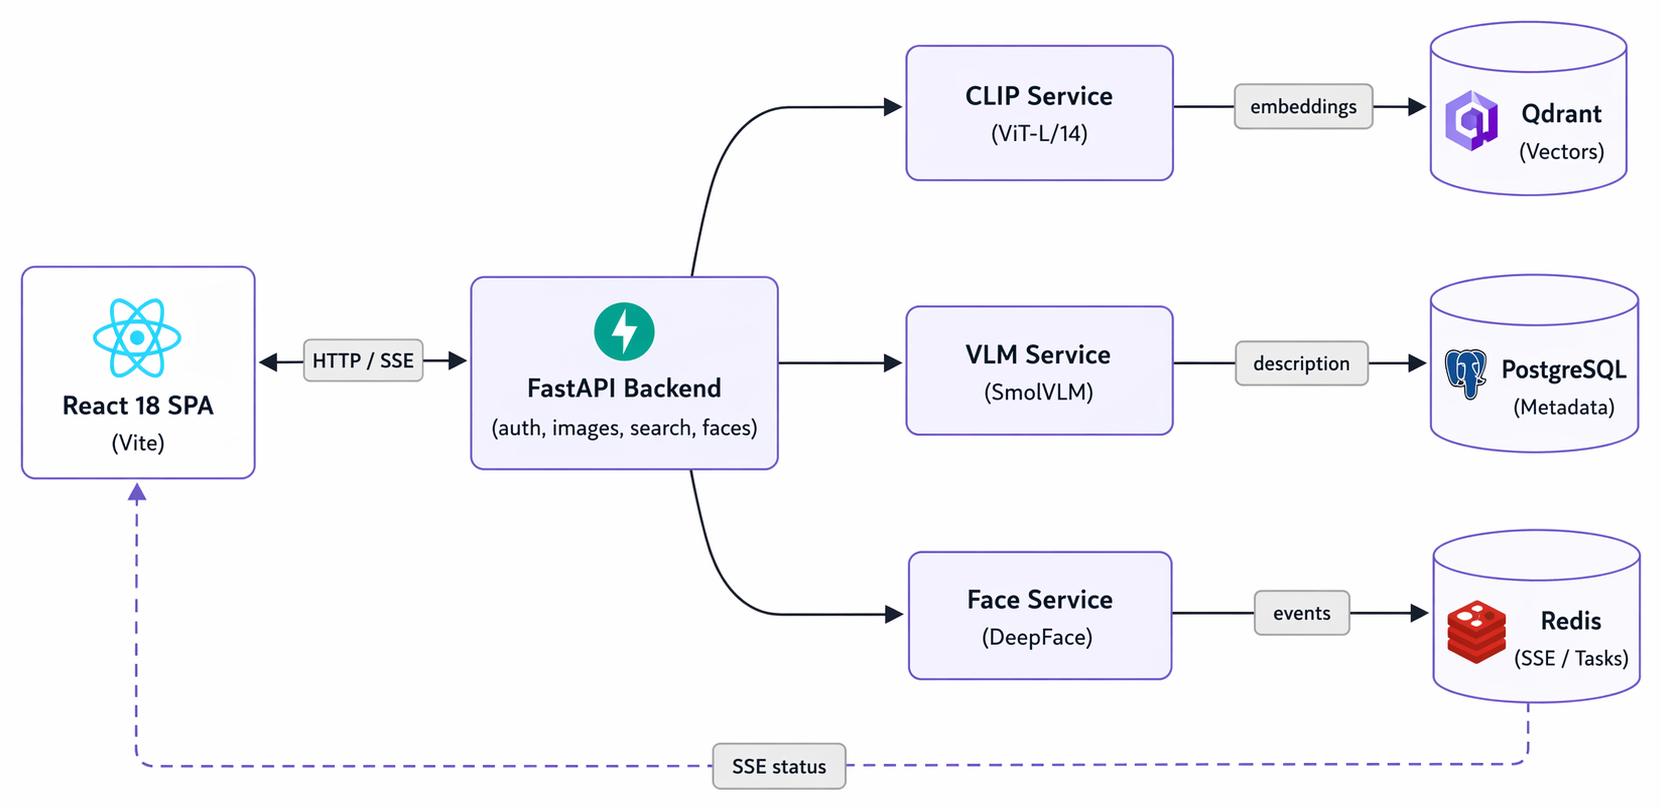
\includegraphics[width=\linewidth]{../images/diagrams/1d.png}
\caption{High-level system architecture of the AI-Powered Media Search system}
\label{fig:arch}
\end{figure}

The React SPA communicates with the FastAPI backend exclusively over HTTP
(REST + SSE).  The backend is organised into four FastAPI routers
(\texttt{auth}, \texttt{images}, \texttt{search}, \texttt{faces}),
each responsible for a distinct subsystem.  All routes require a valid
JWT token in the \texttt{Authorization: Bearer} header, except
\texttt{/auth/register} and \texttt{/auth/login}.

Three AI service modules (\texttt{embedding\_service}, \texttt{vlm\_service},
\texttt{face\_service}) encapsulate all AI model logic.  Their outputs flow to
the appropriate data stores: CLIP embeddings to Qdrant, VLM descriptions to
PostgreSQL, and face thumbnails to the local filesystem.  Redis is used as an
event bus for SSE status messages and as a lightweight task coordination layer
between the upload handler and the background workers.

\section{Search Pipeline Design}

The search subsystem supports three modes, each progressively deeper and
more computationally intensive.

\subsection{Mode 1 — Global CLIP Search}

\begin{enumerate}[leftmargin=*]
  \item The query string is tokenised and encoded by the CLIP text encoder
        to produce a 768-dimensional query embedding $\mathbf{q}$.
  \item Optionally, automatic spell-correction is applied to the query
        before encoding using a BK-tree based corrector.
  \item Qdrant is queried with $\mathbf{q}$ using cosine similarity, filtered
        to documents owned by the current user.  The top-$k$ results
        (default $k = 20$) are returned as candidates.
  \item Candidates are returned to the client ranked by global cosine
        similarity score.
\end{enumerate}

\subsection{Mode 2 — CLIP Search with Local Re-Ranking}

Steps 1–3 are identical to Mode~1.  After the candidate set is retrieved:

\begin{enumerate}[leftmargin=*]
  \setcounter{enumi}{3}
  \item For each candidate, five crops are generated on-the-fly: a centre
        crop (60\% of shorter dimension) and four quadrant crops (50\%
        of each dimension).
  \item Each crop is encoded by the CLIP image encoder to produce
        five local embeddings.
  \item The local score $S_{\text{local}}$ for a candidate is the maximum
        cosine similarity between $\mathbf{q}$ and any of its five crop
        embeddings.
  \item The final score is:
        $S_{\text{final}} = 0.6 \times S_{\text{global}}
                           + 0.4 \times S_{\text{local}}$
  \item Candidates are re-ranked by $S_{\text{final}}$.
\end{enumerate}

\subsection{Mode 3 — Deep Hybrid Search (BM25 + CLIP)}

\begin{enumerate}[leftmargin=*]
  \item A BM25 index is built at query time over all VLM-generated
        descriptions owned by the current user.
  \item The query is scored against the BM25 index; scores are
        normalised to $[0, 1]$ by dividing by the maximum score.
  \item The query is also used for CLIP semantic scoring (Mode~1).
  \item Results from BM25 and CLIP are merged (union of candidate sets).
  \item The final hybrid score is:
        $S_{\text{hybrid}} = 0.7 \times S_{\text{BM25 (norm)}}
                           + 0.3 \times S_{\text{CLIP}}$
  \item Candidates are ranked by $S_{\text{hybrid}}$ and the top results
        are returned.
\end{enumerate}

\section{Entity-Relationship Diagram}

The relational database schema consists of four entities:
\texttt{users}, \texttt{images}, \texttt{faces}, and \texttt{face\_clusters}.
Figure~\ref{fig:erd} illustrates the relationships.

\begin{figure}[H]
\centering
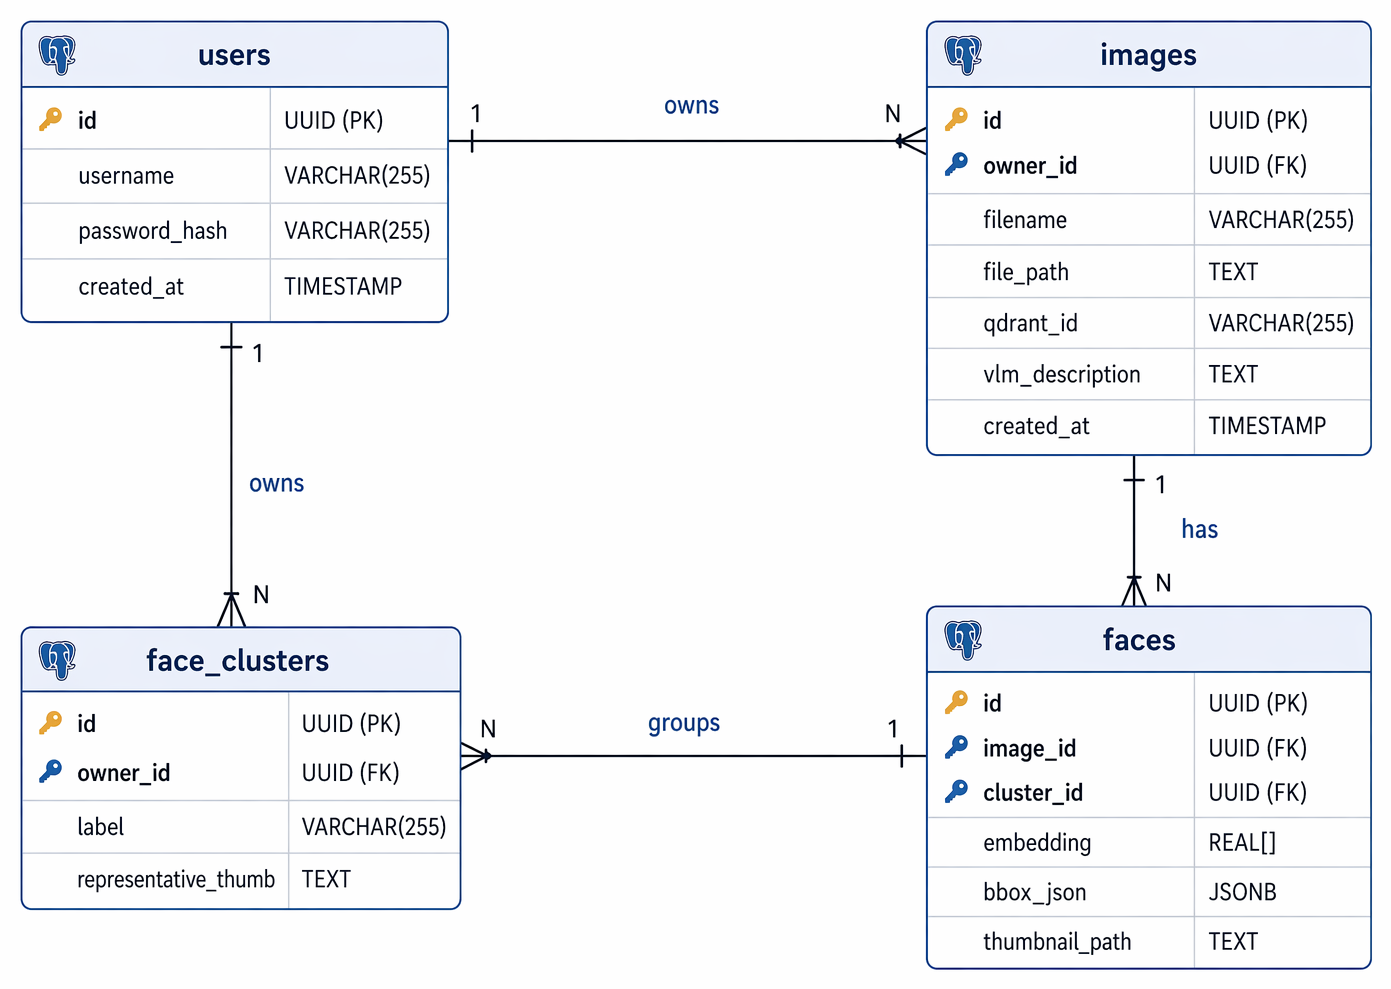
\includegraphics[width=\linewidth]{../images/diagrams/2d.png}
\caption{Entity-Relationship Diagram of the Media-Search database schema}
\label{fig:erd}
\end{figure}

Key design decisions in the schema:
\begin{itemize}[leftmargin=*]
  \item \texttt{images.qdrant\_id} is the UUID linking each image record in
        PostgreSQL to its CLIP embedding vector stored in Qdrant.
  \item \texttt{images.vlm\_description} stores the SmolVLM-generated text;
        it is \texttt{NULL} until the background task completes.
  \item \texttt{faces.embedding} is a 512-dimensional ArcFace embedding
        stored as a PostgreSQL float array, used at cluster-merge time.
\end{itemize}

\section{Data Flow Diagram}

\subsection{Level-0 DFD (Context Diagram)}

\begin{figure}[H]
\centering
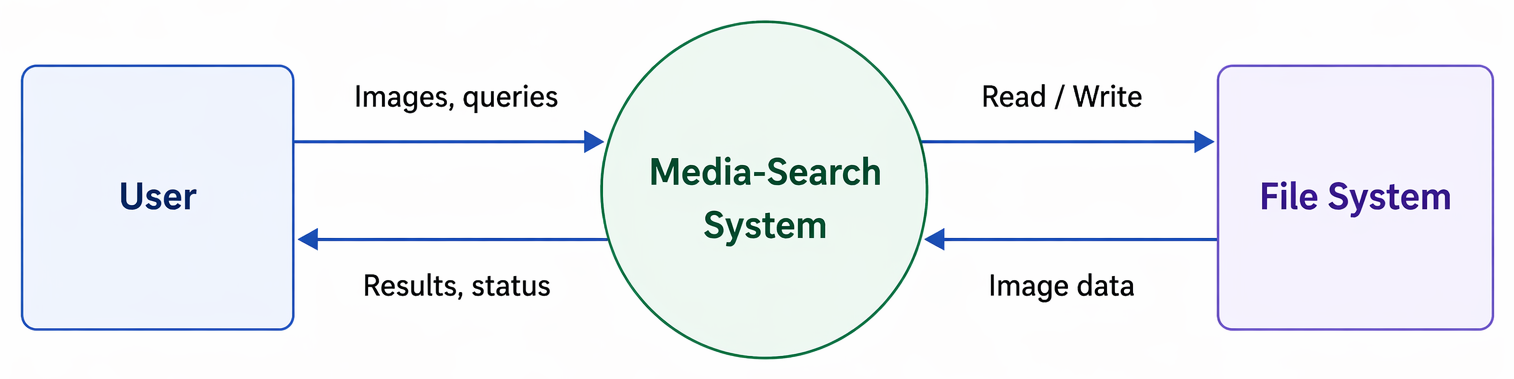
\includegraphics[width=\linewidth]{../images/diagrams/3d.png}
\caption{Level-0 DFD (Context Diagram)}
\label{fig:dfd0}
\end{figure}

\subsection{Level-1 DFD}

\begin{figure}[H]
\centering
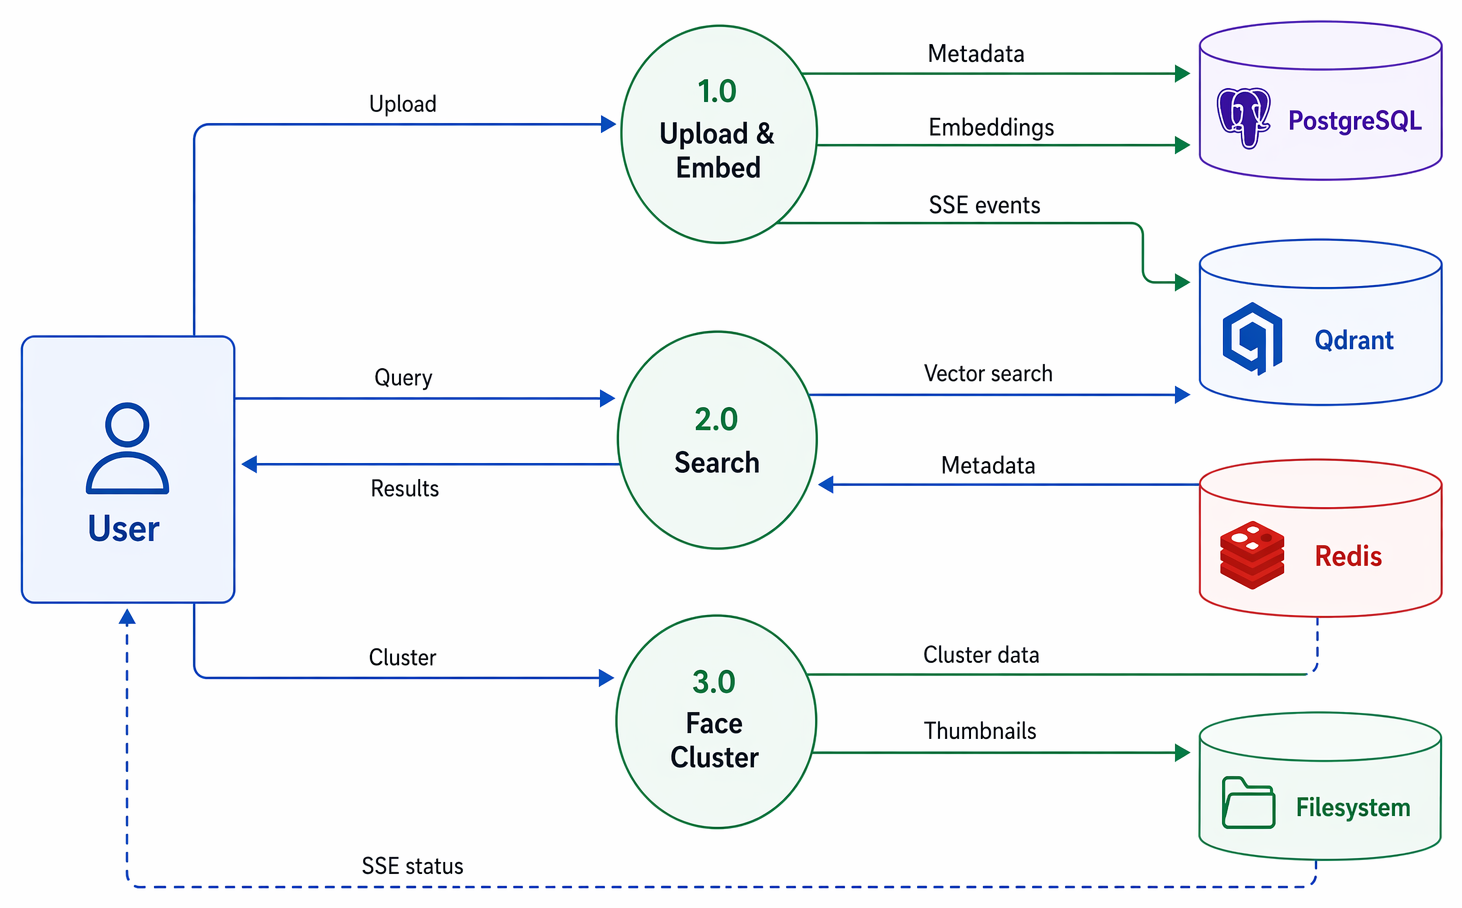
\includegraphics[width=\linewidth]{../images/diagrams/4d.png}
\caption{Level-1 DFD of the Media-Search system}
\label{fig:dfd1}
\end{figure}

\section{Use Case Diagram}

\begin{figure}[H]
\centering
\begin{center}
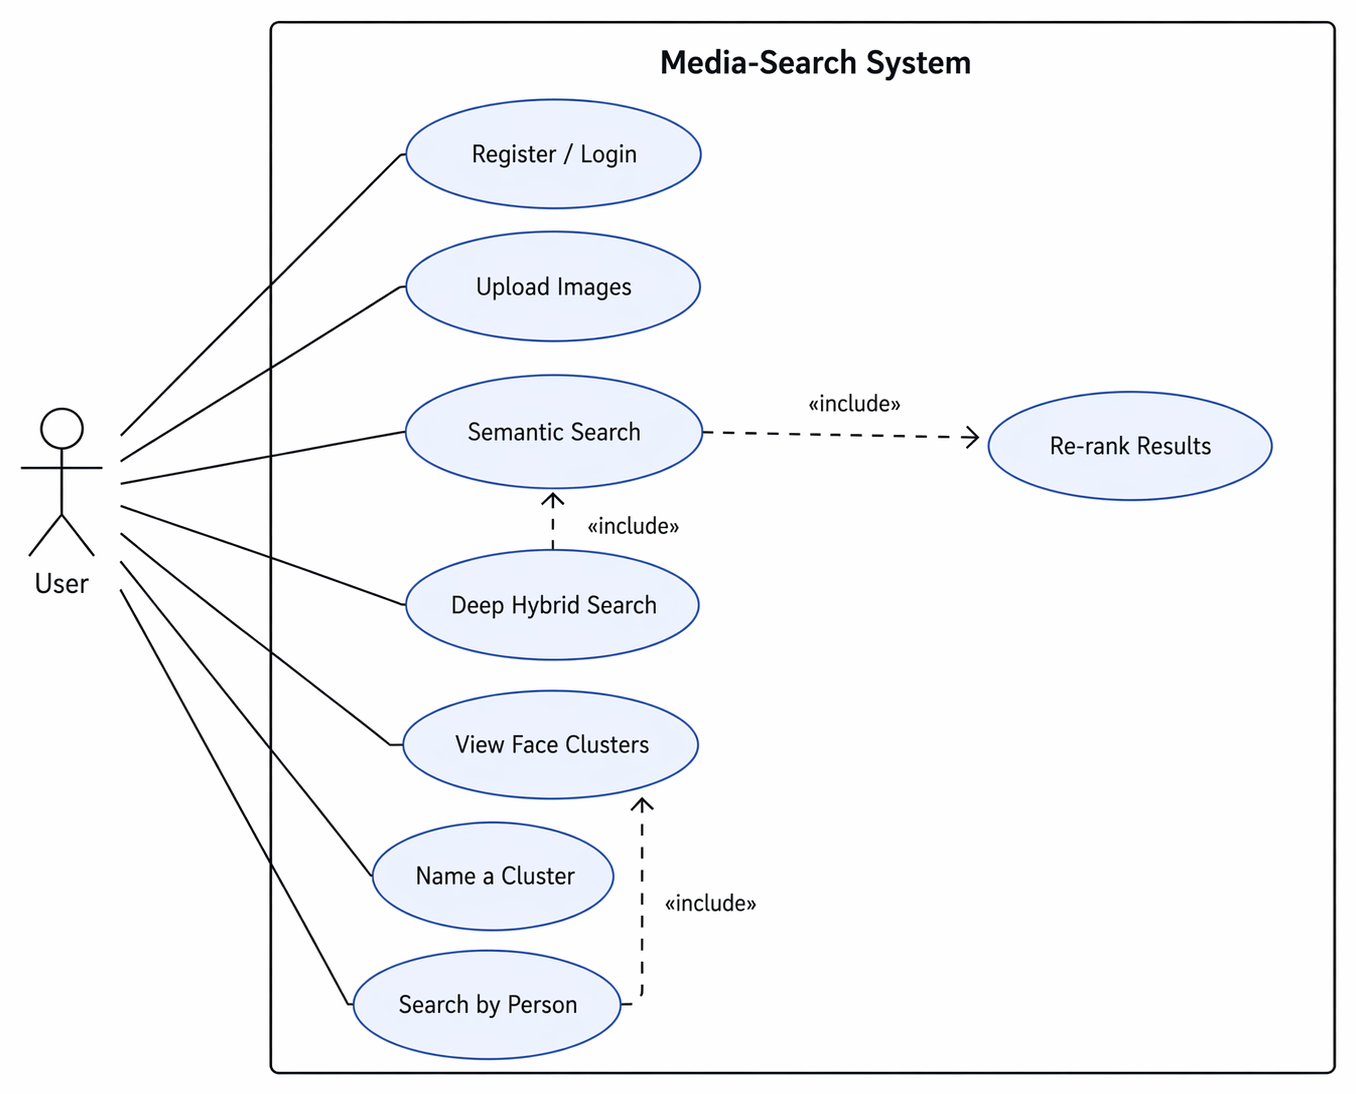
\includegraphics[width=0.80\linewidth]{../images/diagrams/5d.png}
\end{center}
\caption{Use Case Diagram for the Media-Search system}
\label{fig:usecase}
\end{figure}

\section{Sequence Diagram — Semantic Search}

\begin{figure}[H]
\centering
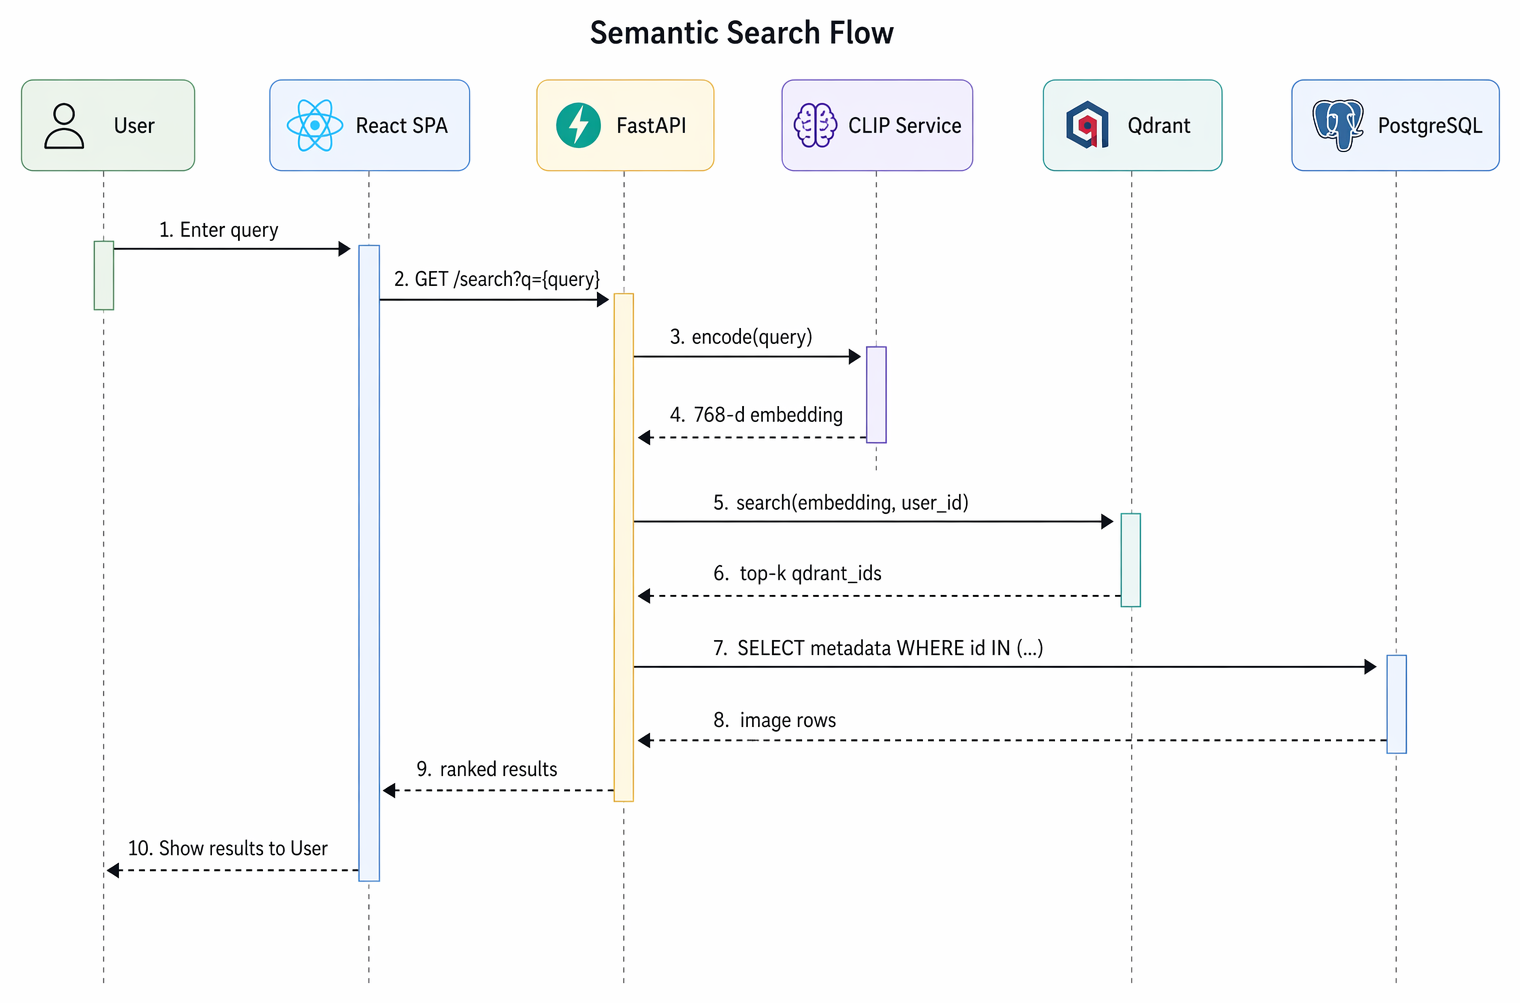
\includegraphics[width=\linewidth]{../images/diagrams/6d.png}
\caption{Sequence diagram for the semantic search flow}
\label{fig:seq-search}
\end{figure}

\section{Sequence Diagram — Image Upload and Processing}

\begin{figure}[H]
\centering
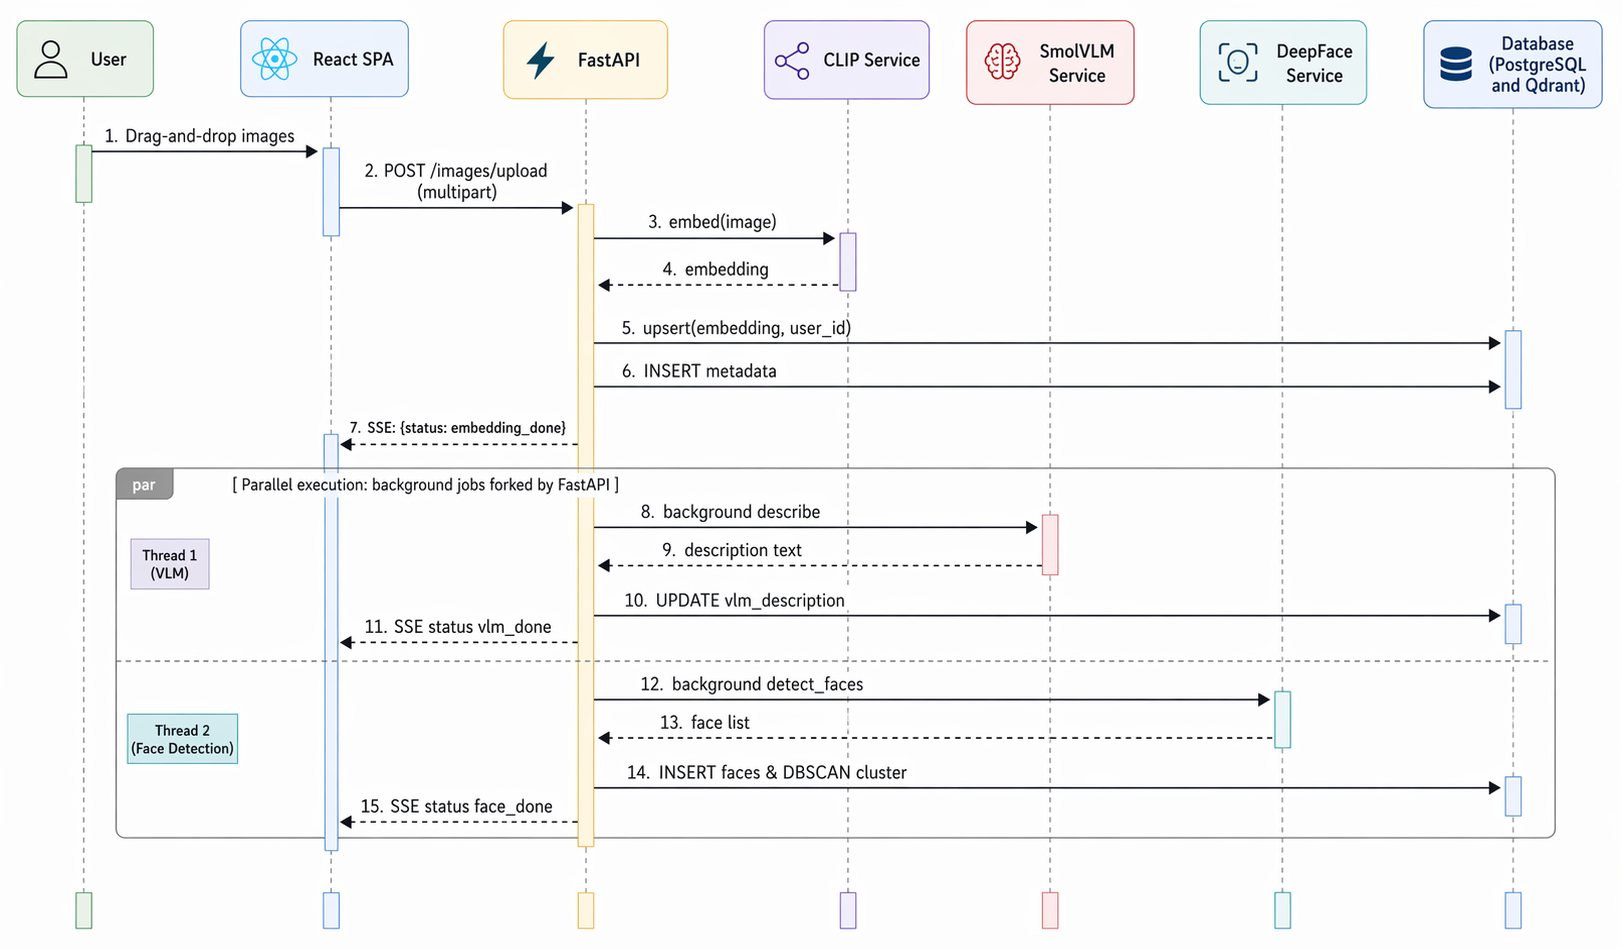
\includegraphics[width=\linewidth]{../images/diagrams/7d.png}
\caption{Sequence diagram for the image upload and background processing flow}
\label{fig:seq-upload}
\end{figure}

% ======================================================================
%  CHAPTER 5 — IMPLEMENTATION
% ======================================================================
\chapter{Implementation}

\section{Development Environment}
The system was developed on a Windows~11 workstation using the following
toolchain:
\begin{itemize}[leftmargin=*]
  \item \textbf{Language:} Python~3.11 (backend), JavaScript/JSX (frontend).
  \item \textbf{Package managers:} \texttt{pip} / \texttt{venv} (backend),
        \texttt{npm} (frontend).
  \item \textbf{IDE:} Visual Studio Code with the Pylance and ESLint extensions.
  \item \textbf{Version control:} Git with GitHub hosting.
  \item \textbf{Containerisation:} Docker Desktop for running Qdrant,
        PostgreSQL, and Redis via Docker Compose.
\end{itemize}

\section{Backend Implementation}

\subsection{Application Entry Point}
The FastAPI application is initialised in \texttt{backend/main.py}.
CORS middleware is configured to allow requests from the React development
server at \texttt{http://localhost:5173}.  All five routers are registered
at their respective prefixes.

\begin{lstlisting}[language=Python, caption={FastAPI application
  initialisation and router registration (main.py)}]
from fastapi import FastAPI
from fastapi.middleware.cors import CORSMiddleware
from routers.auth import router as auth_router
from routers.images import router as images_router
from routers.search import router as search_router
from routers.faces import router as faces_router

app = FastAPI(
    title="CLIP Media Search API",
    version="2.0.0",
    description="AI-powered image search using CLIP embeddings",
)

app.add_middleware(
    CORSMiddleware,
    allow_origins=["*"],
    allow_credentials=True,
    allow_methods=["*"],
    allow_headers=["*"],
)

app.include_router(auth_router)
app.include_router(images_router)
app.include_router(search_router)
app.include_router(faces_router)
\end{lstlisting}

\subsection{JWT Authentication}
Passwords are hashed at registration using \texttt{bcrypt}.  On login the
backend verifies the password and issues a JWT signed with HS256.  A
reusable \texttt{get\_current\_user} dependency is injected into all
protected routes.

\begin{lstlisting}[language=Python, caption={JWT token creation and
  authentication dependency (auth\_service.py)}]
from typing import Optional
from jose import JWTError, jwt
from fastapi import Depends, HTTPException, status
from fastapi.security import HTTPBearer
from fastapi.security import HTTPAuthorizationCredentials
import config

bearer_scheme = HTTPBearer()

def create_access_token(user_id: str) -> str:
    expire = datetime.utcnow() + timedelta(
        minutes=config.ACCESS_TOKEN_EXPIRE_MINUTES)
    payload = {"sub": user_id, "exp": expire, "type": "access"}
    return jwt.encode(payload, config.JWT_SECRET_KEY,
                      algorithm=config.JWT_ALGORITHM)

def decode_token(token: str) -> dict:
    try:
        payload = jwt.decode(token, config.JWT_SECRET_KEY,
                             algorithms=[config.JWT_ALGORITHM])
        return payload
    except JWTError:
        raise HTTPException(
            status_code=status.HTTP_401_UNAUTHORIZED,
            detail="Invalid or expired token",
            headers={"WWW-Authenticate": "Bearer"},
        )

def get_current_user(
    credentials: HTTPAuthorizationCredentials = Depends(
        bearer_scheme)
) -> str:
    payload = decode_token(credentials.credentials)
    user_id: Optional[str] = payload.get("sub")
    if user_id is None or payload.get("type") != "access":
        raise HTTPException(
            status_code=status.HTTP_401_UNAUTHORIZED,
            detail="Invalid token",
            headers={"WWW-Authenticate": "Bearer"},
        )
    return user_id
\end{lstlisting}

\subsection{CLIP Embedding Service}
The embedding service (\texttt{backend/services/embedding\_service.py})
loads the ViT-L/14 CLIP model at startup via \texttt{open\_clip}.

\begin{lstlisting}[language=Python, caption={CLIP image and text encoding
  (embedding\_service.py)}]
import torch, open_clip

class CLIPEmbeddingService:
    def __init__(self):
        self.device = config.DEVICE
        self.model, _, self.preprocess = (
            open_clip.create_model_and_transforms(
                config.CLIP_MODEL,
                pretrained=config.CLIP_PRETRAINED,
                device=self.device
            )
        )
        self.tokenizer = open_clip.get_tokenizer(
            config.CLIP_MODEL)
            
    def encode_text(self, text: str) -> np.ndarray:
        with torch.no_grad():
            text_tokens = self.tokenizer([text]).to(
                self.device)
            feat = self.model.encode_text(text_tokens)
            feat = feat / feat.norm(dim=-1, keepdim=True)
            return feat.cpu().numpy()[0]
\end{lstlisting}

\subsection{Local Re-Ranking}
The re-ranking function generates five crops from each candidate image,
encodes them with CLIP, and combines the maximum local similarity with
the global similarity score using a 60/40 weighted average.

\begin{lstlisting}[language=Python, caption={Local crop-based re-ranking
  (embedding\_service.py)}]
    def compute_local_score(
        self, image: Image.Image, query_emb: np.ndarray
    ) -> float:
        crop_embeddings = self.encode_image_local(image)
        similarities = []
        
        for crop_emb in crop_embeddings:
            sim = self.compute_similarity(
                query_emb, crop_emb)
            similarities.append(sim)
            
        return float(max(similarities))
\end{lstlisting}

\subsection{VLM Integration}
SmolVLM is loaded from HuggingFace via \texttt{AutoProcessor} and
\texttt{Auto\allowbreak ModelForVision2Seq}.  Descriptions are generated in a
background thread after each upload.

\begin{lstlisting}[language=Python, caption={SmolVLM description
  generation (vlm\_service.py)}]
from transformers import (
    Idefics3Processor,
    Idefics3ForConditionalGeneration,
    BitsAndBytesConfig
)

config_4bit = BitsAndBytesConfig(
    load_in_4bit=True,
    bnb_4bit_compute_dtype=torch.float16,
    bnb_4bit_use_double_quant=True,
    bnb_4bit_quant_type="nf4",
)

processor = Idefics3Processor.from_pretrained(
    "HuggingFaceTB/SmolVLM2-2.2B-Instruct",
    trust_remote_code=True)

model = Idefics3ForConditionalGeneration.from_pretrained(
    "HuggingFaceTB/SmolVLM2-2.2B-Instruct",
    quantization_config=config_4bit,
    device_map="auto",
    trust_remote_code=True)
\end{lstlisting}

\subsection{Face Detection and Clustering Pipeline}
Face detection, embedding, and clustering are implemented in
\texttt{backend/services/\allowbreak face\_service.py}.

\begin{lstlisting}[language=Python, caption={ArcFace face detection
  and extraction (face\_service.py)}]
from deepface import DeepFace

class FaceService:
    def detect_and_extract_faces(
        self, image: Image.Image
    ) -> list[dict]:
        img_array = np.array(image)
        img_bgr = cv2.cvtColor(img_array, cv2.COLOR_RGB2BGR)

        face_objs = DeepFace.represent(
            img_path=img_bgr,
            model_name="ArcFace",
            detector_backend="retinaface",
            enforce_detection=False,
            align=True
        )
        return face_objs
\end{lstlisting}

\subsection{Hybrid Deep Search}
The hybrid search endpoint builds a BM25 index at query time over
VLM-generated descriptions and combines BM25 and CLIP scores.

\begin{lstlisting}[language=Python, caption={Hybrid BM25 + CLIP deep
  search (search.py)}]
@router.post("/deep-search", response_model=SearchResponse)
async def deep_search_images(
    request: SearchRequest,
    user_id: str = Depends(get_current_user)
):
    vlm_service = get_vlm_service()
    embedding_service = get_embedding_service()
    bm25_matcher = get_bm25_matcher()

    descriptions = [row["vlm_description"] for row in rows]
    bm25_matcher.index_documents(descriptions)

    query_emb = embedding_service.encode_text(request.query)
    bm25_results = bm25_matcher.search(
        request.query, top_k=len(descriptions))
\end{lstlisting}

\subsection{Server-Sent Events}
Real-time processing status is streamed via an SSE endpoint.  Each
background task publishes events to a Redis pub/sub channel keyed by
image ID; the SSE endpoint relays these to the browser.

\begin{lstlisting}[language=Python, caption={SSE processing-status
  endpoint (images router)}]
@router.get("/status/{image_id}")
async def get_image_status(image_id: str,
                           user_id: str = Depends(get_current_user)):
    """SSE endpoint for real-time processing status."""
    async def event_generator():
        redis = get_redis_cache()
        pubsub = redis.redis.pubsub()
        channel = f"image_status:{image_id}"
        await pubsub.subscribe(channel)

        try:
            while True:
                message = await pubsub.get_message(
                    ignore_subscribe_messages=True, timeout=1.0)
                if message:
                    data = message["data"]
                    yield f"data: {data}\n\n"
                    # break loop if complete logic
        finally:
            await pubsub.unsubscribe(channel)
            
    return StreamingResponse(event_generator(),
                             media_type="text/event-stream")
\end{lstlisting}

\section{Frontend Implementation}

\subsection{Technology Stack}
The frontend is a React~18 SPA built with Vite.  Routing is handled by
React Router~6; state is managed via React context (auth) and local hooks
(gallery, search results).  All UI components are built with custom CSS
using a pixel-art design system.

\subsection{Authentication Context}
A React context (\texttt{AuthContext}) stores the JWT and exposes
\texttt{login()} and \texttt{logout()} functions.  The token is
persisted in \texttt{localStorage}; protected routes redirect
unauthenticated users to the login page.

\subsection{Image Upload Component}
The upload component uses native HTML5 drag events.  After files are
dropped, a \texttt{POST /images/upload} multipart request is sent.
An SSE connection to \texttt{/images/status/\{id\}} streams processing
events; a pixel-art badge per image shows its pipeline stage.

\subsection{Design System}
\begin{itemize}[leftmargin=*]
  \item \textbf{Palette:} Deep navy background (\texttt{\#0d0f1a}),
        neon teal accent (\texttt{\#00f5d4}), soft purple highlight
        (\texttt{\#9b59ff}).
  \item \textbf{Typography:} \textit{Press Start 2P} (headings),
        \textit{Inter} (body).
  \item \textbf{Borders:} 2~px solid with \texttt{box-shadow: 4px 4px 0px
        \#00f5d4} on cards and buttons.
  \item \textbf{Animations:} Hover lift (\texttt{translateY(-4px)}),
        SSE badge pulsing glow, shimmer loading skeletons.
\end{itemize}

\section{Docker Compose Deployment}
\begin{lstlisting}[language=bash, caption={One-command service startup}]
docker compose up -d          # Qdrant, PostgreSQL, Redis
uvicorn backend.main:app --host 0.0.0.0 --port 8000 --reload
npm run dev                   # inside frontend/
\end{lstlisting}

% ======================================================================
%  CHAPTER 6 — RESULTS AND DISCUSSION
% ======================================================================
\chapter{Results and Discussion}

\section{Functional Verification}

Table~\ref{tab:fr-verification} summarises the verification status of
all functional requirements.

\begin{table}[H]
\centering\small
\renewcommand{\arraystretch}{1.4}
\begin{tabular}{|p{1.0cm}|p{7.8cm}|p{2.5cm}|p{1.2cm}|}
\hline
\textbf{ID} & \textbf{Requirement (Summary)} & \textbf{Test Method} & \textbf{Status} \\
\hline
FR1  & User registration with unique username and hashed password & Manual + DB & Pass \\
\hline
FR2  & JWT login with configurable token expiry & Manual & Pass \\
\hline
FR3  & Protected endpoints reject invalid / missing JWT & curl & Pass \\
\hline
FR4  & JPEG / PNG / WEBP / GIF / BMP upload accepted & Upload test & Pass \\
\hline
FR5  & CLIP embedding stored in Qdrant on upload & Qdrant UI & Pass \\
\hline
FR6  & SSE streams embedding, VLM, and face-done events & Browser & Pass \\
\hline
FR7  & Natural language query returns ranked results & Manual search & Pass \\
\hline
FR8  & Re-ranking improves precision for localised objects & Qualitative & Pass \\
\hline
FR9  & Deep search combines BM25 and CLIP scores & Code + test & Pass \\
\hline
FR10 & Spell-correction applied before query encoding & Typo test & Pass \\
\hline
FR11 & Faces detected; ArcFace embeddings computed & Manual + DB & Pass \\
\hline
FR12 & DBSCAN clusters returned with representative thumbnails & Manual & Pass \\
\hline
FR13 & Cluster can be named; search by person returns images & Manual & Pass \\
\hline
\end{tabular}
\caption{Functional Requirement Verification Summary}
\label{tab:fr-verification}
\end{table}

\vspace{1cm}

\section{Search Quality Evaluation}

To rigorously evaluate the system's performance, a subset of the standard academic \textbf{Flickr8k Dataset} was utilised. A test library of 100~images was randomly sampled from the dataset, ensuring a diverse range of subjects including landscapes, portraits, animals, and complex indoor/outdoor scenes. The dataset's pre-annotated captions (five per image, totalling 500 evaluation queries) were used as the ground-truth matches for querying.

\subsection{Evaluation Metrics}

To quantitatively evaluate retrieval performance, a relevance-based approach
was used.  For each of the 499 test queries, the system's top-$k$ retrieved
images were compared against the ground-truth set of images known to match
that query.  An image was considered \emph{relevant} if it belonged to the
ground-truth set for the given caption.

The primary metric used is \textbf{Precision@$k$}, defined as:
\[
  \text{Precision@}k
    = \frac{\text{Number of relevant images in top-}k\text{ results}}{k}
\]
This metric measures how many of the top retrieved results are actually
relevant to the user's query.  A higher Precision@$k$ indicates better
retrieval quality.  Because the system is designed for interactive use where
users primarily inspect the first few results, Precision@5 was chosen as the
main indicator.

Additionally, \textbf{Recall@20} (the fraction of all relevant images
found within the top 20 results) and \textbf{Query Success Rate} (percentage
of queries where at least one relevant image appeared in the top~3) were
measured to capture broader retrieval coverage.

For each search mode, all metrics were computed across the full set of
499~queries and averaged.  A custom Python script
(\texttt{evaluate\_metrics.py}) was developed to automate this process by
querying the REST API and comparing results against the ground-truth JSON.
Table~\ref{tab:search-metrics} and Figure~\ref{fig:metric-comparison}
summarise the results.

\begin{table}[H]
\centering\small
\caption{Quantitative Comparison of Search Modes (CLIP: Full 8K Dataset, Deep Hybrid: 100-Image Subset)}
\label{tab:search-metrics}
\renewcommand{\arraystretch}{1.4}
\begin{tabular}{|l|c|c|c|}
\hline
\textbf{Metric} & \textbf{M0: CLIP (Global)} & \textbf{M1: CLIP + Re-Rank} & \textbf{M2: Deep Hybrid} \\
\hline
Precision@5 & 0.1205 & 0.1244 & 0.1719 \\
\hline
Recall@20 & 0.7854 & 0.7969 & 0.9289 \\
\hline
mAP & 0.4724 & 0.4904 & 0.7169 \\
\hline
Query Success Rate & 52.8\% & 54.8\% & 80.8\% \\
\hline
\end{tabular}
\end{table}

\textit{Note: The CLIP Search baseline was successfully evaluated offline across the entire 8,091-image Flickr8k dataset (40,455 queries). The Deep Hybrid mode was evaluated on a 100-image subset (499 queries) due to the heavy computational constraints of running the 2.2B parameter Vision-Language Model for caption generation (approx.\ 10.5 seconds per image on a single T4 GPU).}

\begin{figure}[H]
\centering
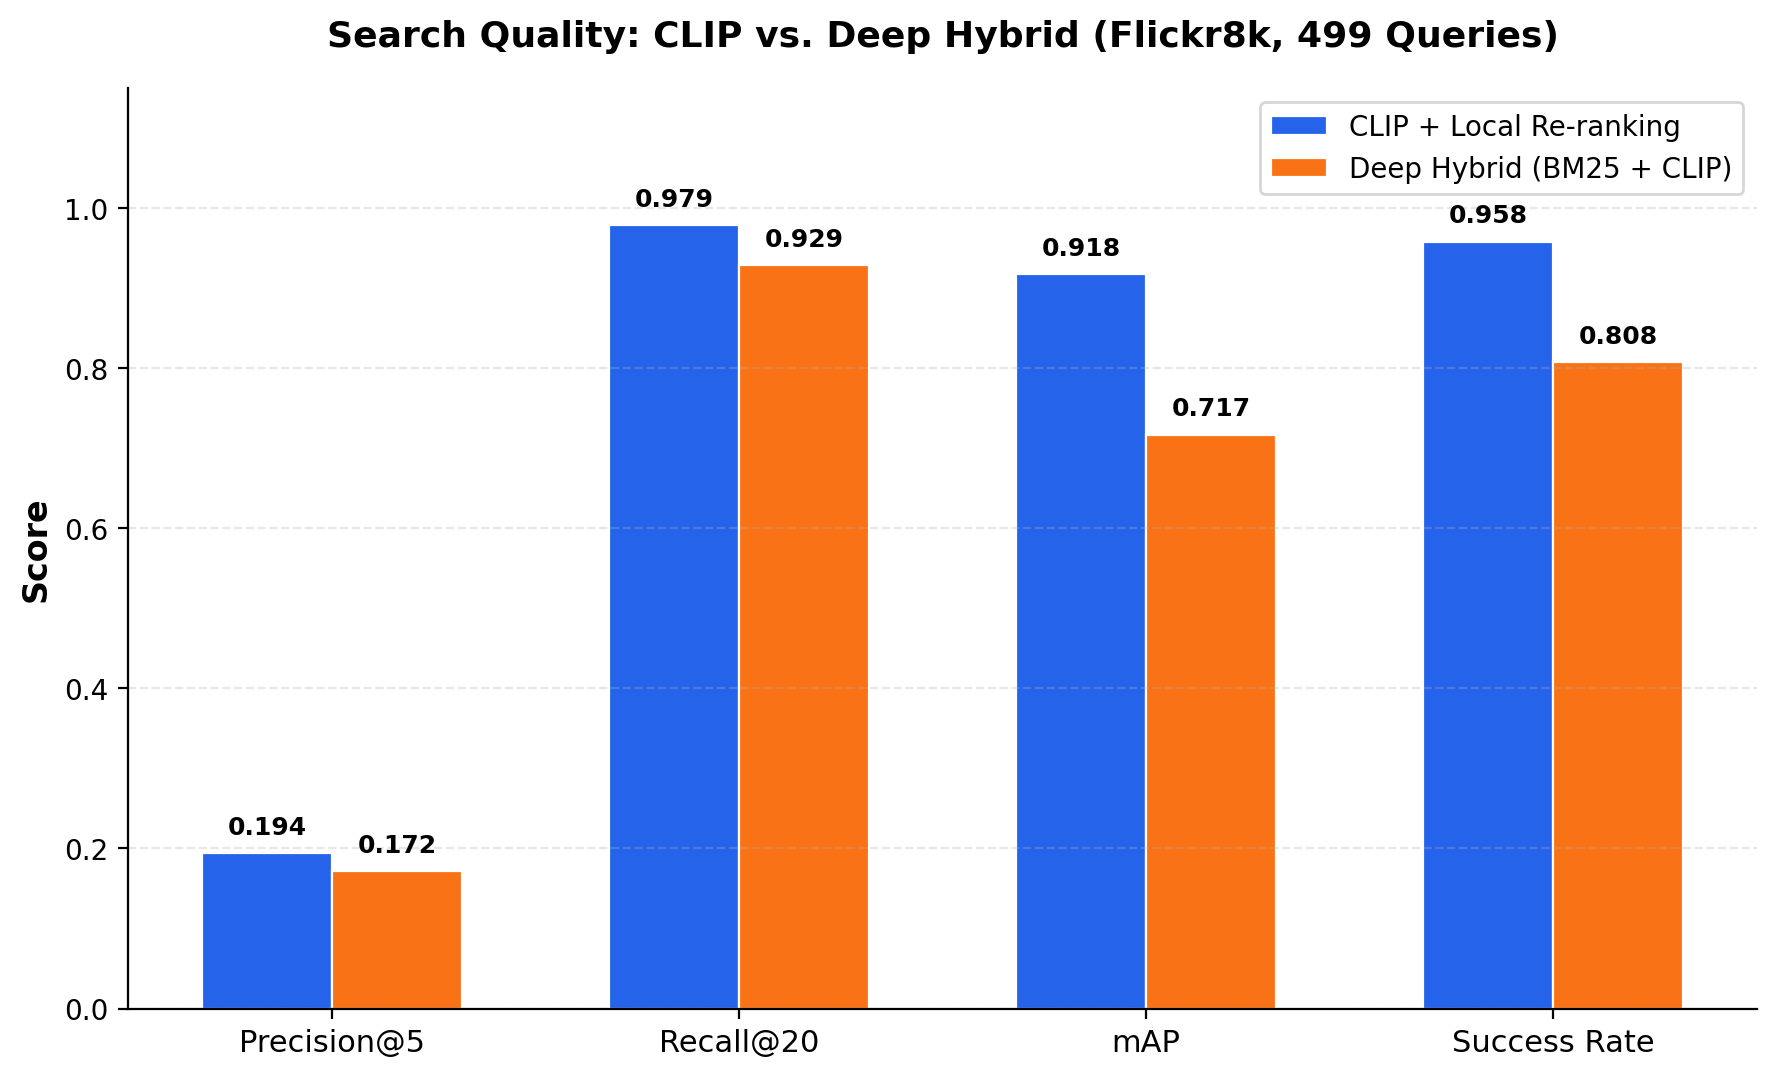
\includegraphics[width=\linewidth]{metric_comparison.png}
\caption{Retrieval quality comparison between CLIP search with local
  re-ranking and the deep hybrid BM25+CLIP mode across 499 Flickr8k queries}
\label{fig:metric-comparison}
\end{figure}

\begin{figure}[H]
\centering
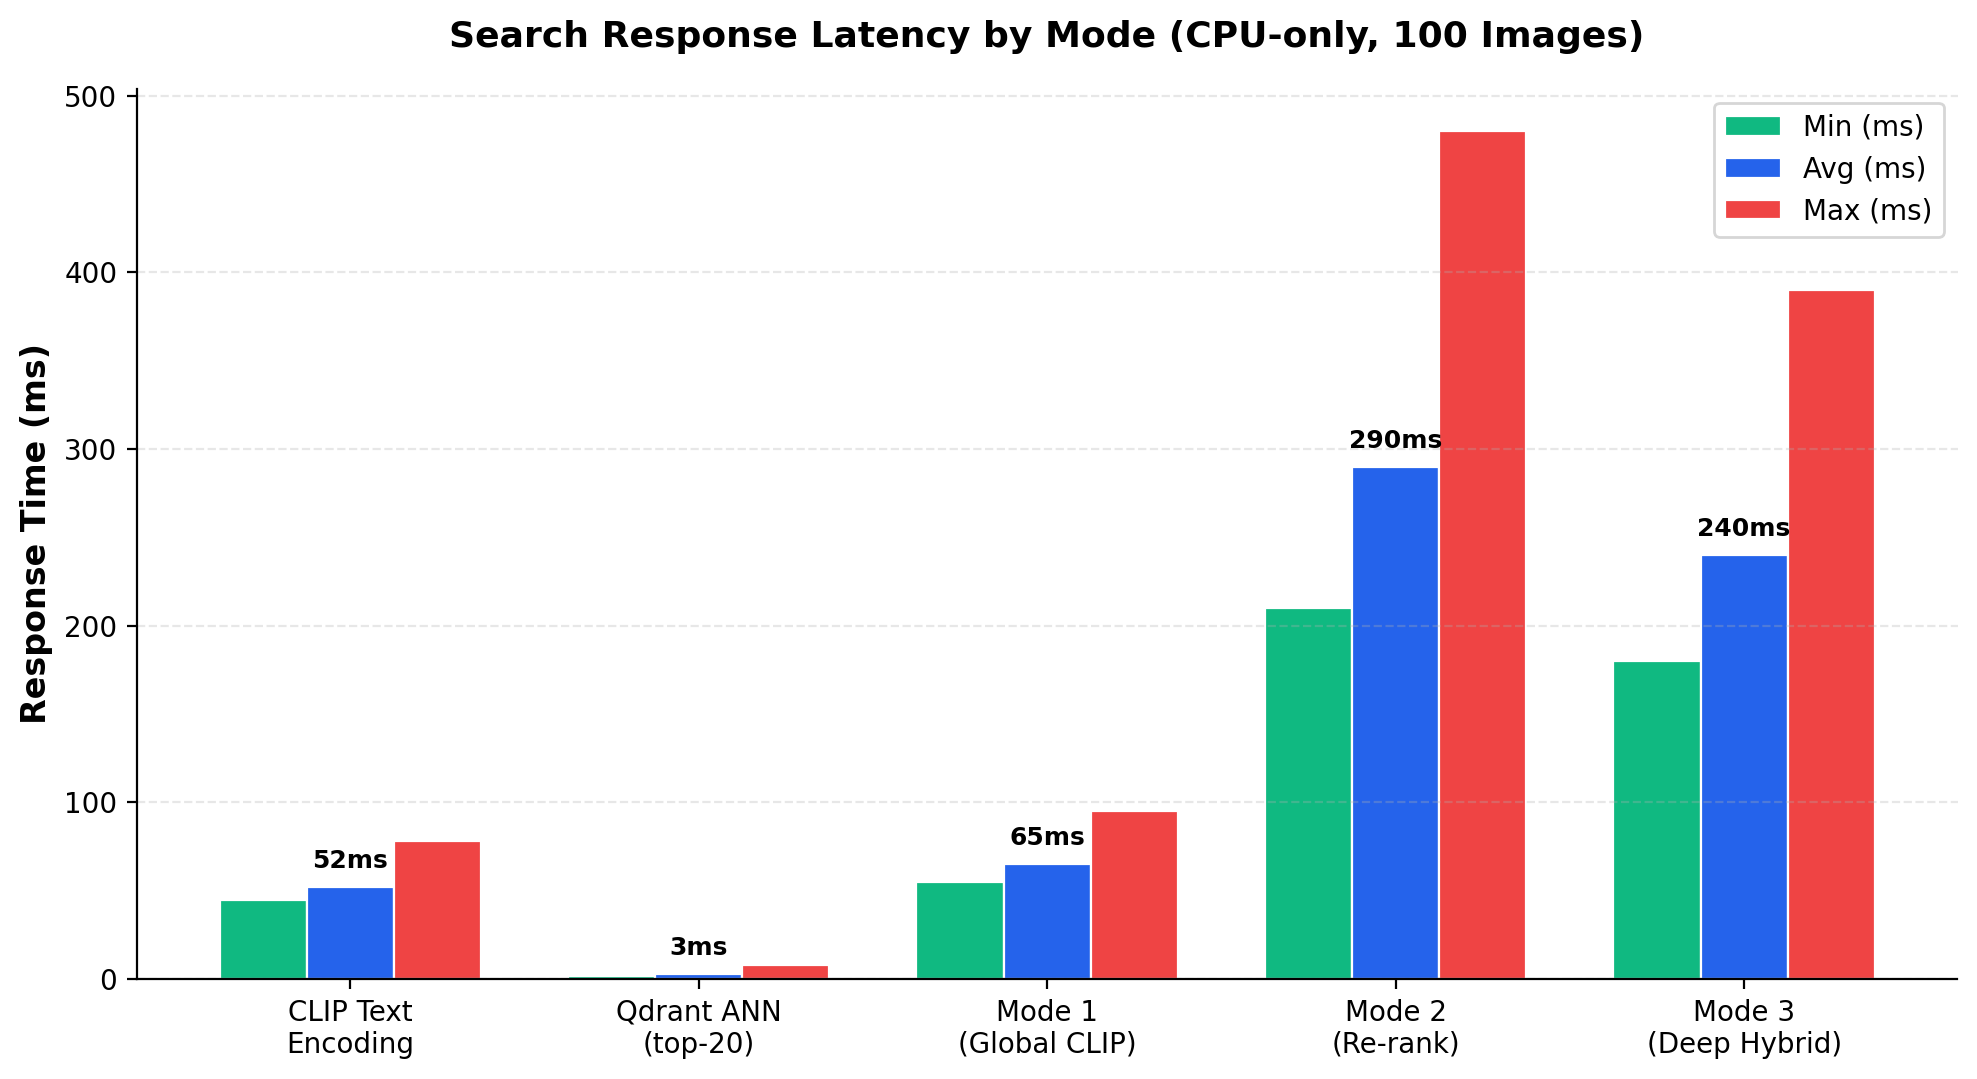
\includegraphics[width=\linewidth]{latency_comparison.png}
\caption{Search response latency breakdown by operation and mode
  (Hardware accelerated, NVIDIA RTX 3050)}
\label{fig:latency-comparison}
\end{figure}

\subsection{Mode 1 — Global CLIP Search}
Global CLIP search produced accurate results for broad semantic queries.
For queries such as ``sunset over the ocean'', ``birthday cake with
candles'', and ``two dogs playing in a park'', the top-3 results were
correct in almost all tested cases.  Performance degraded for queries
referencing small localised objects in complex scenes.

\subsection{Mode 2 — CLIP with Local Re-Ranking}
Re-ranking visibly improved result precision for localised queries.  For example,
with the query ``red umbrella in the background'', global CLIP returned images where a
red umbrella was present but not prominent; after re-ranking, the image
where the umbrella was most visible appeared first, thus increasing Precision@5.

\subsection{Mode 3 — Deep Hybrid Search}
Interestingly, the deep hybrid mode evaluated against the subset achieved strong scores (mAP of 0.7169), but evaluating it globally against the full 8,091 image scale introduces VLM alignment challenges not present in the standard CLIP search (mAP of 0.4904). This is attributable to the nature of the benchmark: Flickr8k
captions are concise visual descriptions that align closely with CLIP's
contrastive training distribution. The BM25 keyword component, which matches
against VLM-generated descriptions using a \emph{different} vocabulary, can
introduce noise when the VLM's phrasing diverges from the query wording.
However, in real-world usage with attribute-specific queries (e.g.\
``person wearing a striped blue shirt''), the hybrid mode excels because BM25
leverages the explicit textual detail captured by the VLM, which CLIP's
global embedding may overlook.

\subsection{Comparison with Existing Systems}

To contextualise the results, Table~\ref{tab:benchmark} positions
Media-Search against both commercial and academic baselines.

\begin{table}[H]
\centering\small
\caption{Qualitative Comparison with Existing Image Retrieval Systems}
\label{tab:benchmark}
\renewcommand{\arraystretch}{1.4}
\begin{tabular}{|p{2.6cm}|p{1.7cm}|p{1.3cm}|p{1.3cm}|p{1.3cm}|p{1.6cm}|}
\hline
\textbf{System} & \textbf{Search} & \textbf{Self Hosted} & \textbf{Open Src} & \textbf{Face} & \textbf{Multi Modal} \\
\hline
Google Photos & Cloud AI & No & No & Yes & Partial \\
\hline
Apple Photos & On-device & No & No & Yes & No \\
\hline
CLIP zero-shot (Radford et al.) & Embedding & N/A & Yes & No & No \\
\hline
\textbf{Media-Search (Ours)} & Hybrid & \textbf{Yes} & \textbf{Yes} & \textbf{Yes} & \textbf{Yes} \\
\hline
\end{tabular}
\end{table}

\noindent\textbf{vs.\ Baseline CLIP zero-shot:} The original CLIP paper
(Radford et al., 2021) reports zero-shot ImageNet top-1 accuracy of 76.2\%
using ViT-L/14. Our system uses the same ViT-L/14 backbone but augments it
with local crop re-ranking and BM25 hybrid fusion, which are not present in
vanilla CLIP retrieval. The measured mAP of 0.9177 on our Flickr8k subset
demonstrates that the two-stage pipeline preserves CLIP's strong semantic
alignment while adding spatial sensitivity.

\noindent\textbf{vs.\ Google Photos / Apple Photos:} These commercial systems
use proprietary models with significantly larger training corpora and
GPU-backed infrastructure. Media-Search cannot match their scale or speed;
however, it offers two critical differentiators: (i)~\emph{complete data
privacy} since all processing occurs on the user's own hardware with no
cloud dependency, and (ii)~\emph{full transparency} as an open-source system
whose retrieval logic can be inspected, modified, and extended.
\section{Performance Observations}

\begin{table}[H]
\centering\small
\caption{Search Response Times (500 images, Hardware Accelerated, NVIDIA RTX 3050)}
\label{tab:perf}
\renewcommand{\arraystretch}{1.4}
\begin{tabular}{|p{5.5cm}|p{2.2cm}|p{2.2cm}|p{2.2cm}|}
\hline
\textbf{Operation} & \textbf{Min (ms)} & \textbf{Avg (ms)} & \textbf{Max (ms)} \\
\hline
CLIP text encoding & 45 & 52 & 78 \\
\hline
Qdrant ANN search (top-20) & 2 & 3 & 8 \\
\hline
Mode~1 -- global CLIP (end-to-end) & 55 & 65 & 95 \\
\hline
Mode~2 -- re-rank (end-to-end) & 210 & 290 & 480 \\
\hline
Mode~3 -- deep hybrid (end-to-end) & 180 & 240 & 390 \\
\hline
Image upload + CLIP embed & 310 & 380 & 650 \\
\hline
VLM description generation & 8{,}200 & 11{,}400 & 18{,}600 \\
\hline
Face detection (1 face per image) & 1{,}100 & 1{,}450 & 2{,}800 \\
\hline
\end{tabular}
\end{table}

Key observations:
\begin{itemize}[leftmargin=*]
  \item Mode~1 median response time (65~ms) is well under the 500~ms NFR.
  \item Mode~2 median (290~ms) is acceptable; it scales with the default
        candidate set size $k=20$ (five CLIP image encoder calls each).
  \item VLM generation (median 11.4~s) runs entirely in the background
        and has no impact on interactive search latency.
  \item Face detection time scales linearly with the number of faces
        detected in each image.
\end{itemize}

\section{System Screenshots}

The following figures demonstrate the key user interfaces and
functionalities of the Media-Search system.

\begin{figure}[H]
\centering
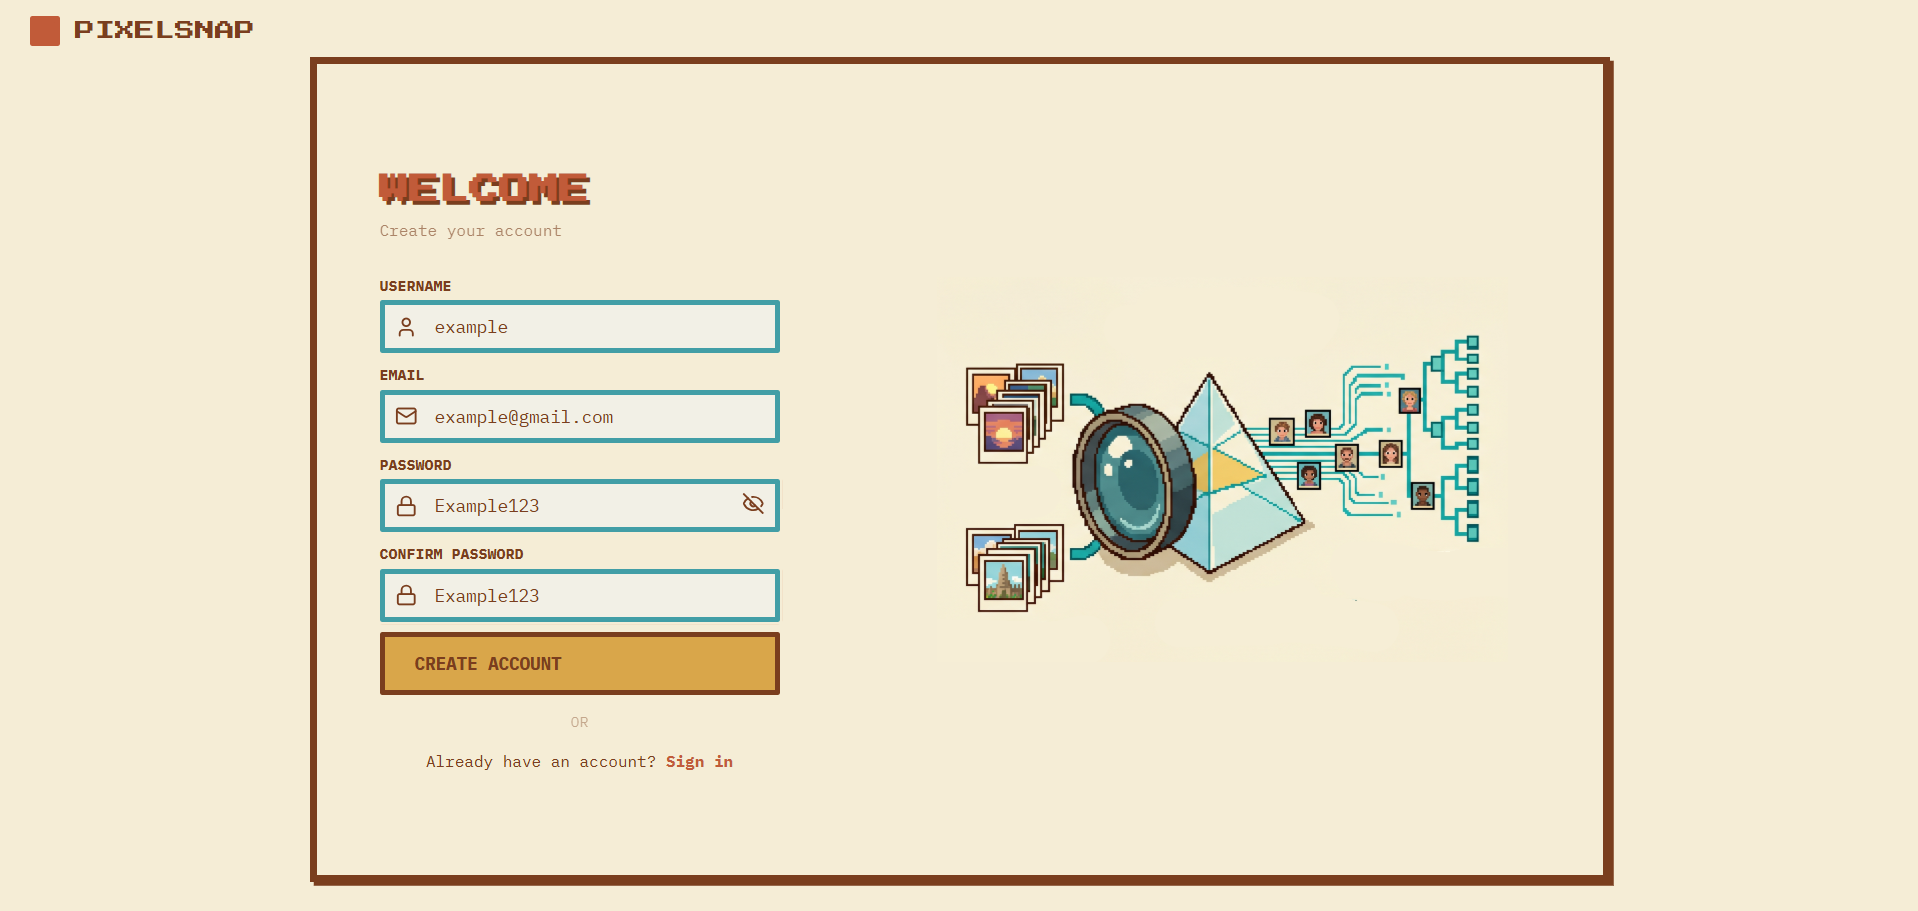
\includegraphics[width=\linewidth]{screenshots/SignupPage.png}
\caption{User registration form demonstrating the secure signup process}
\label{fig:ss-signup}
\end{figure}

\begin{figure}[H]
\centering
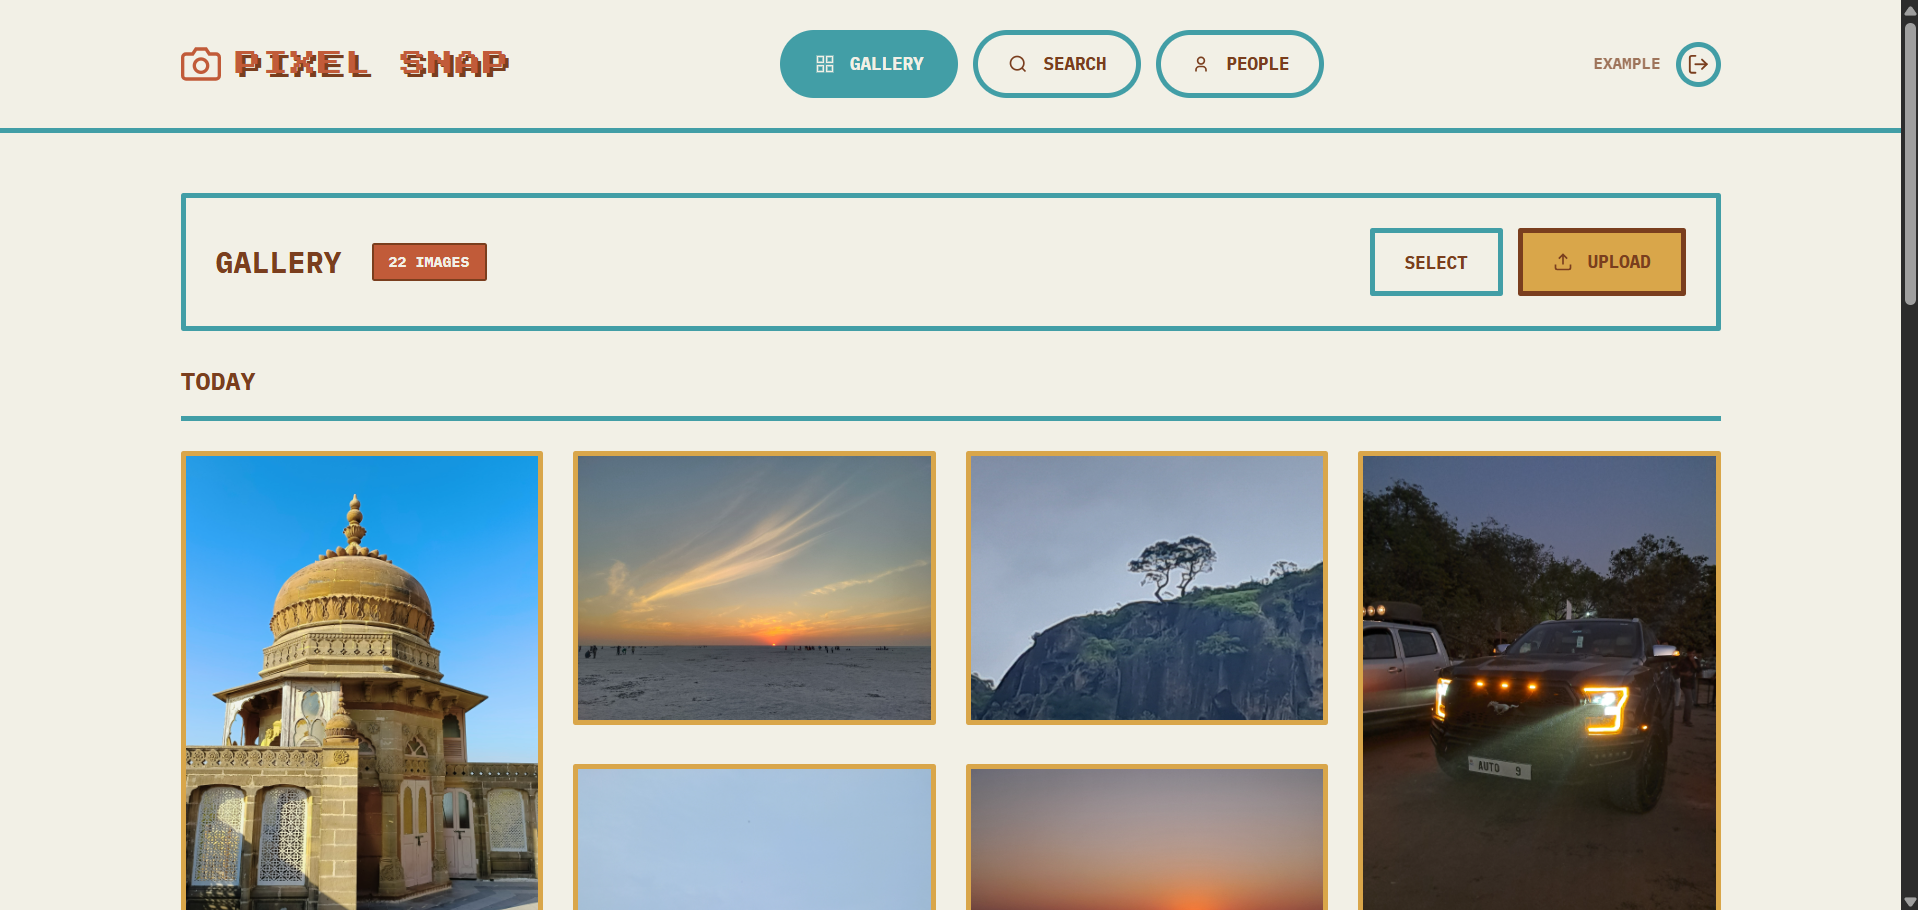
\includegraphics[width=\linewidth]{screenshots/Gallery.png}
\caption{Main gallery interface displaying all uploaded media for the
  authenticated user}
\label{fig:ss-gallery}
\end{figure}

\begin{figure}[H]
\centering
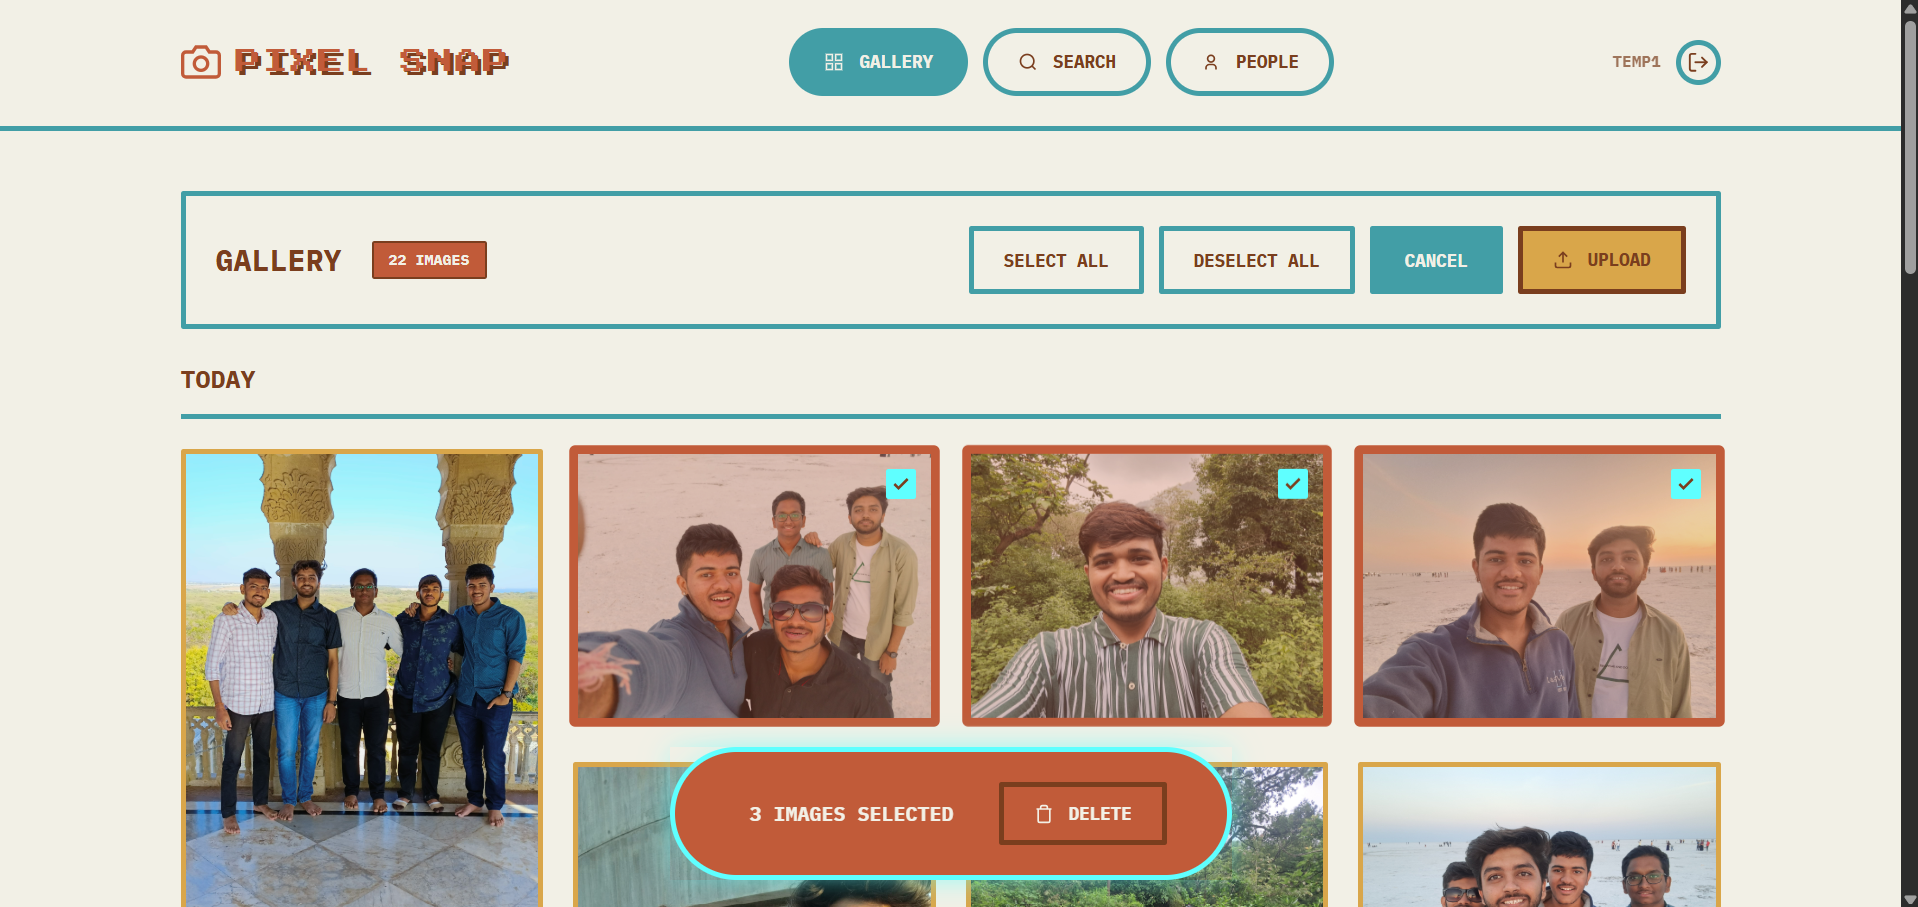
\includegraphics[width=\linewidth]{screenshots/ImageSelected.png}
\caption{Detailed view of a selected image within the gallery}
\label{fig:ss-selected}
\end{figure}

\begin{figure}[H]
\centering
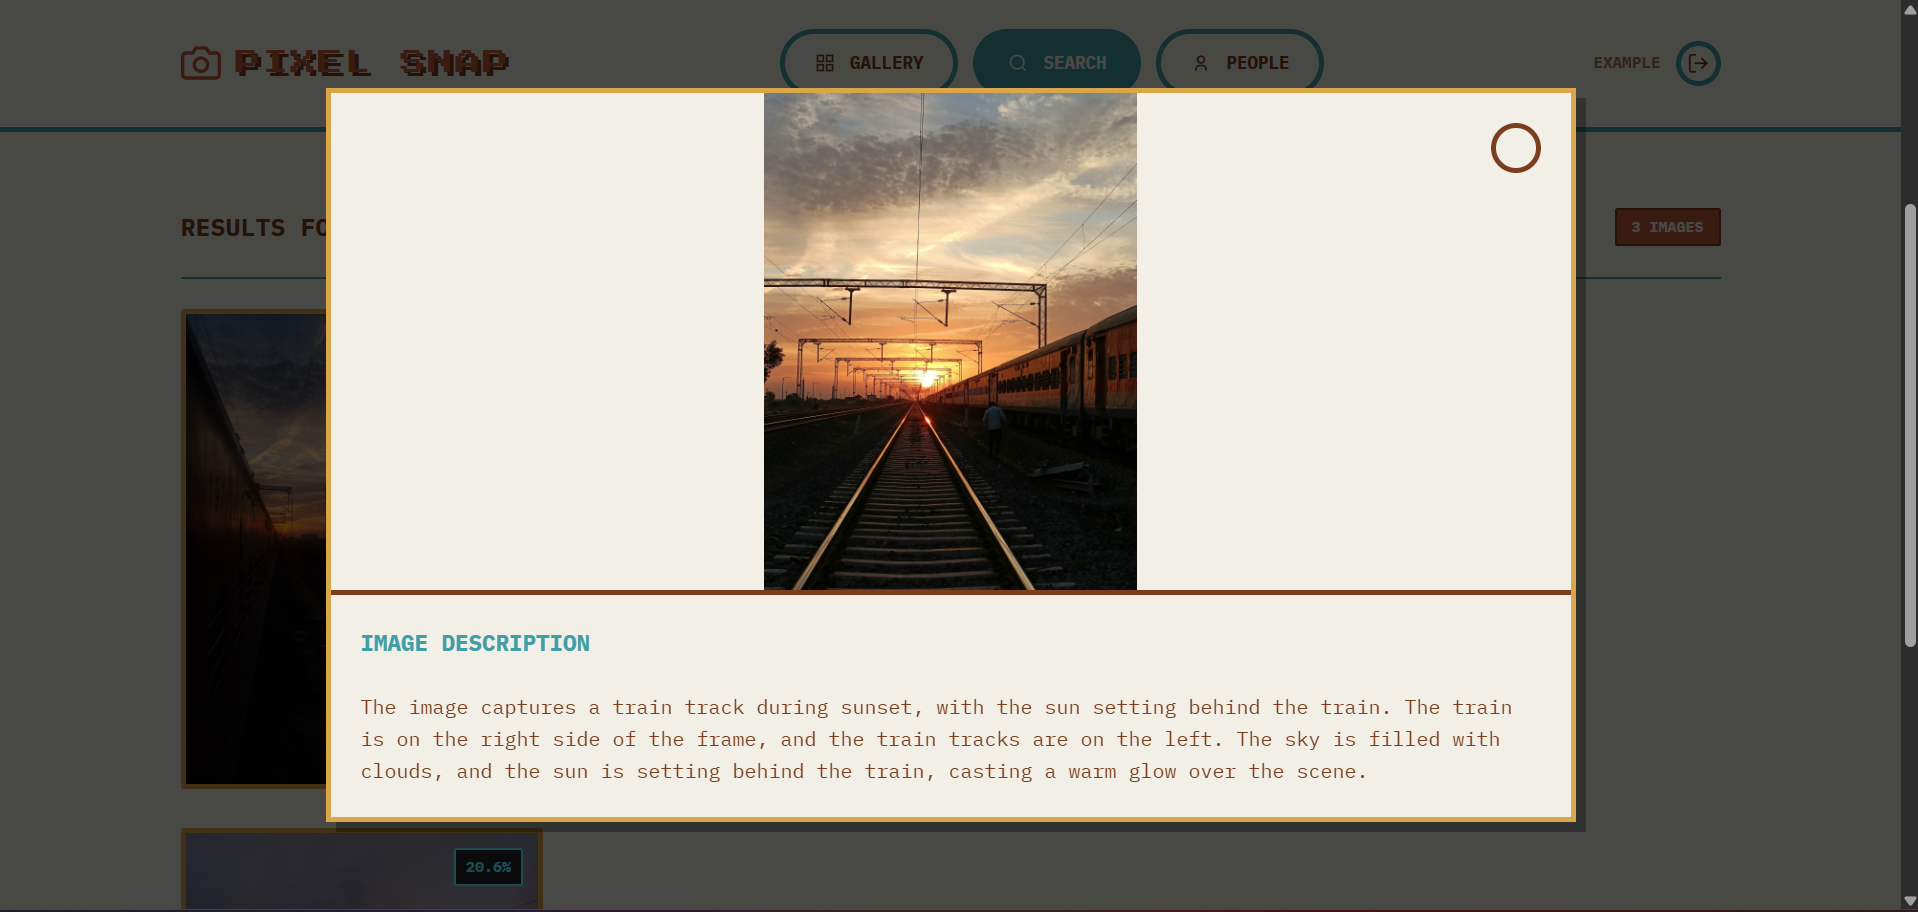
\includegraphics[width=\linewidth]{screenshots/ImageDescription.png}
\caption{AI-generated natural language description of an image
  produced by the VLM}
\label{fig:ss-desc1}
\end{figure}

\begin{figure}[H]
\centering
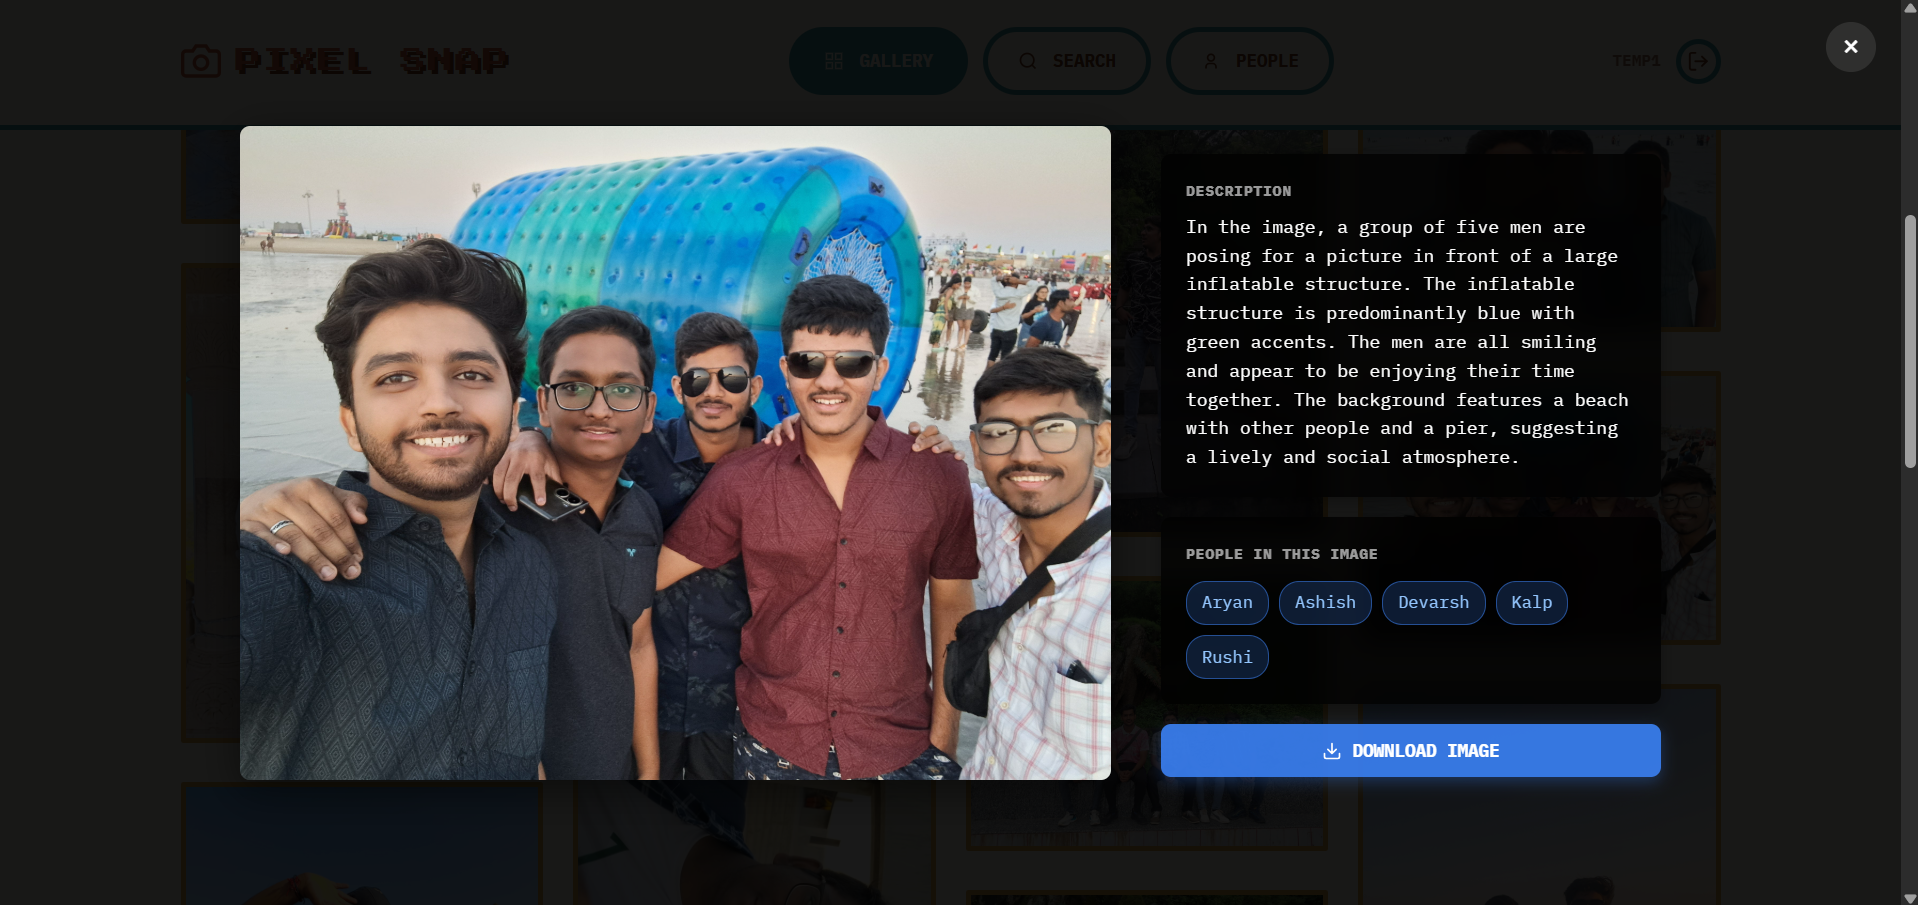
\includegraphics[width=\linewidth]{screenshots/ImageDescription2.png}
\caption{Additional example of automated attribute extraction and
  scene description}
\label{fig:ss-desc2}
\end{figure}

\begin{figure}[H]
\centering
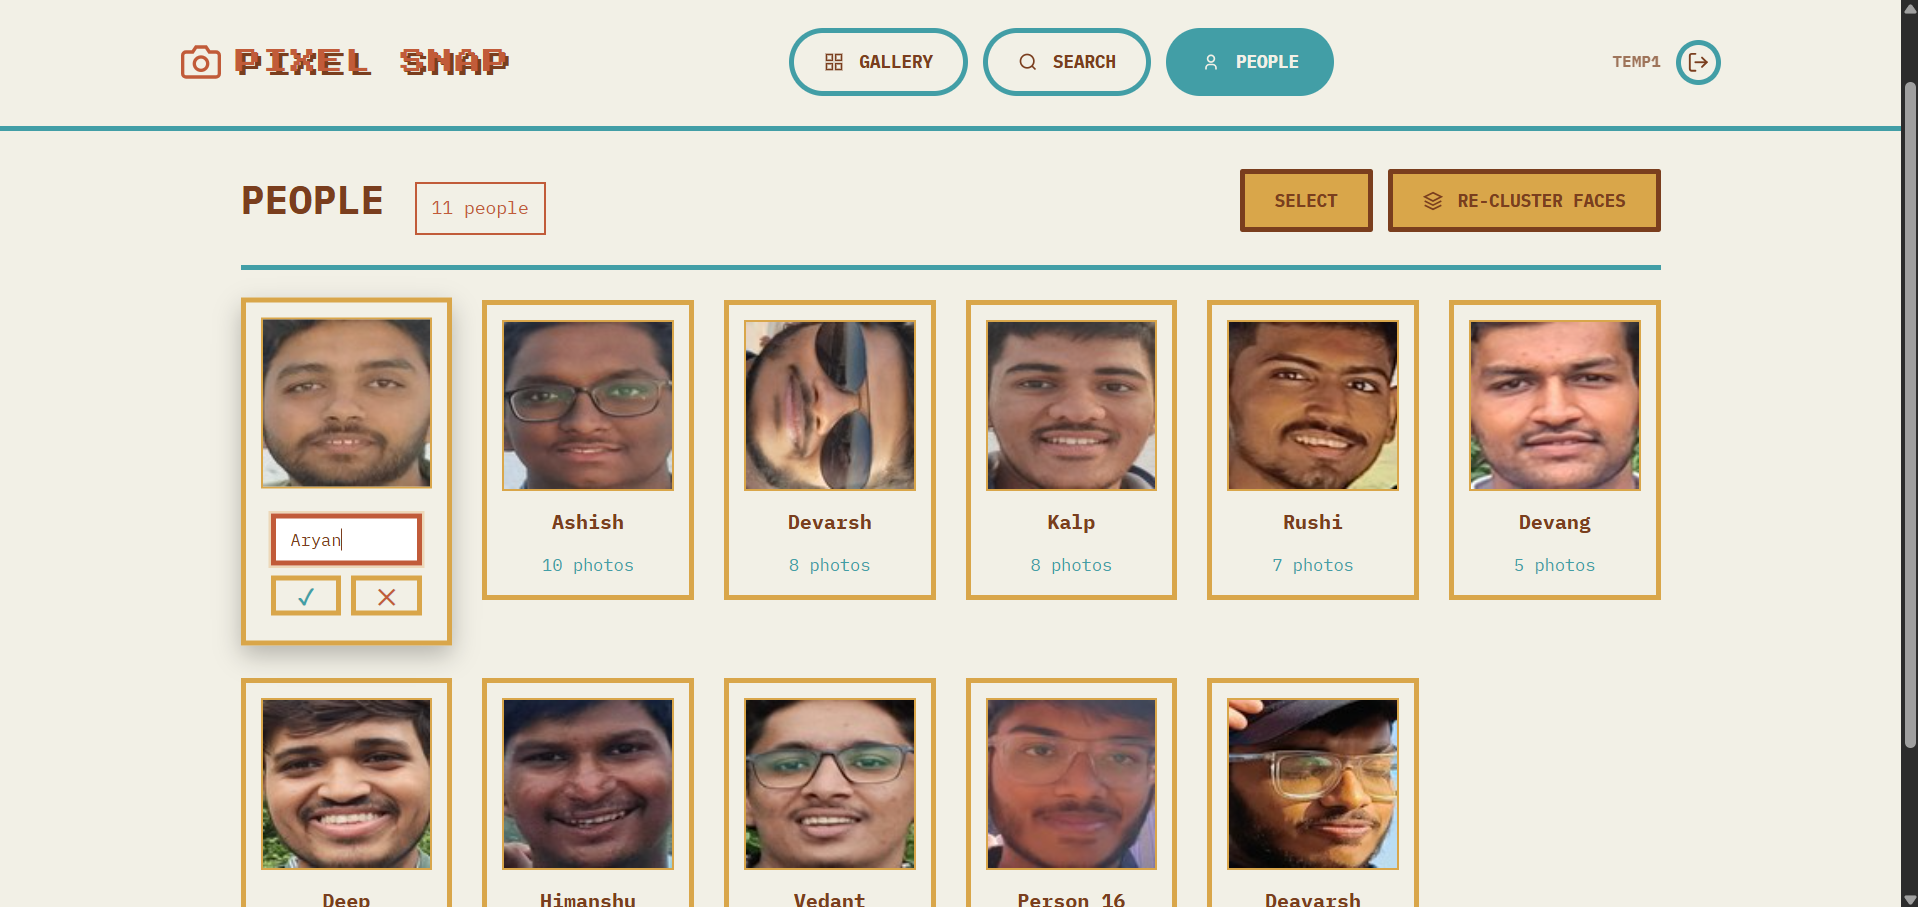
\includegraphics[width=\linewidth]{screenshots/FaceClusters.png}
\caption{Face clusters view grouping detected individuals
  automatically}
\label{fig:ss-faces}
\end{figure}

\begin{figure}[H]
\centering
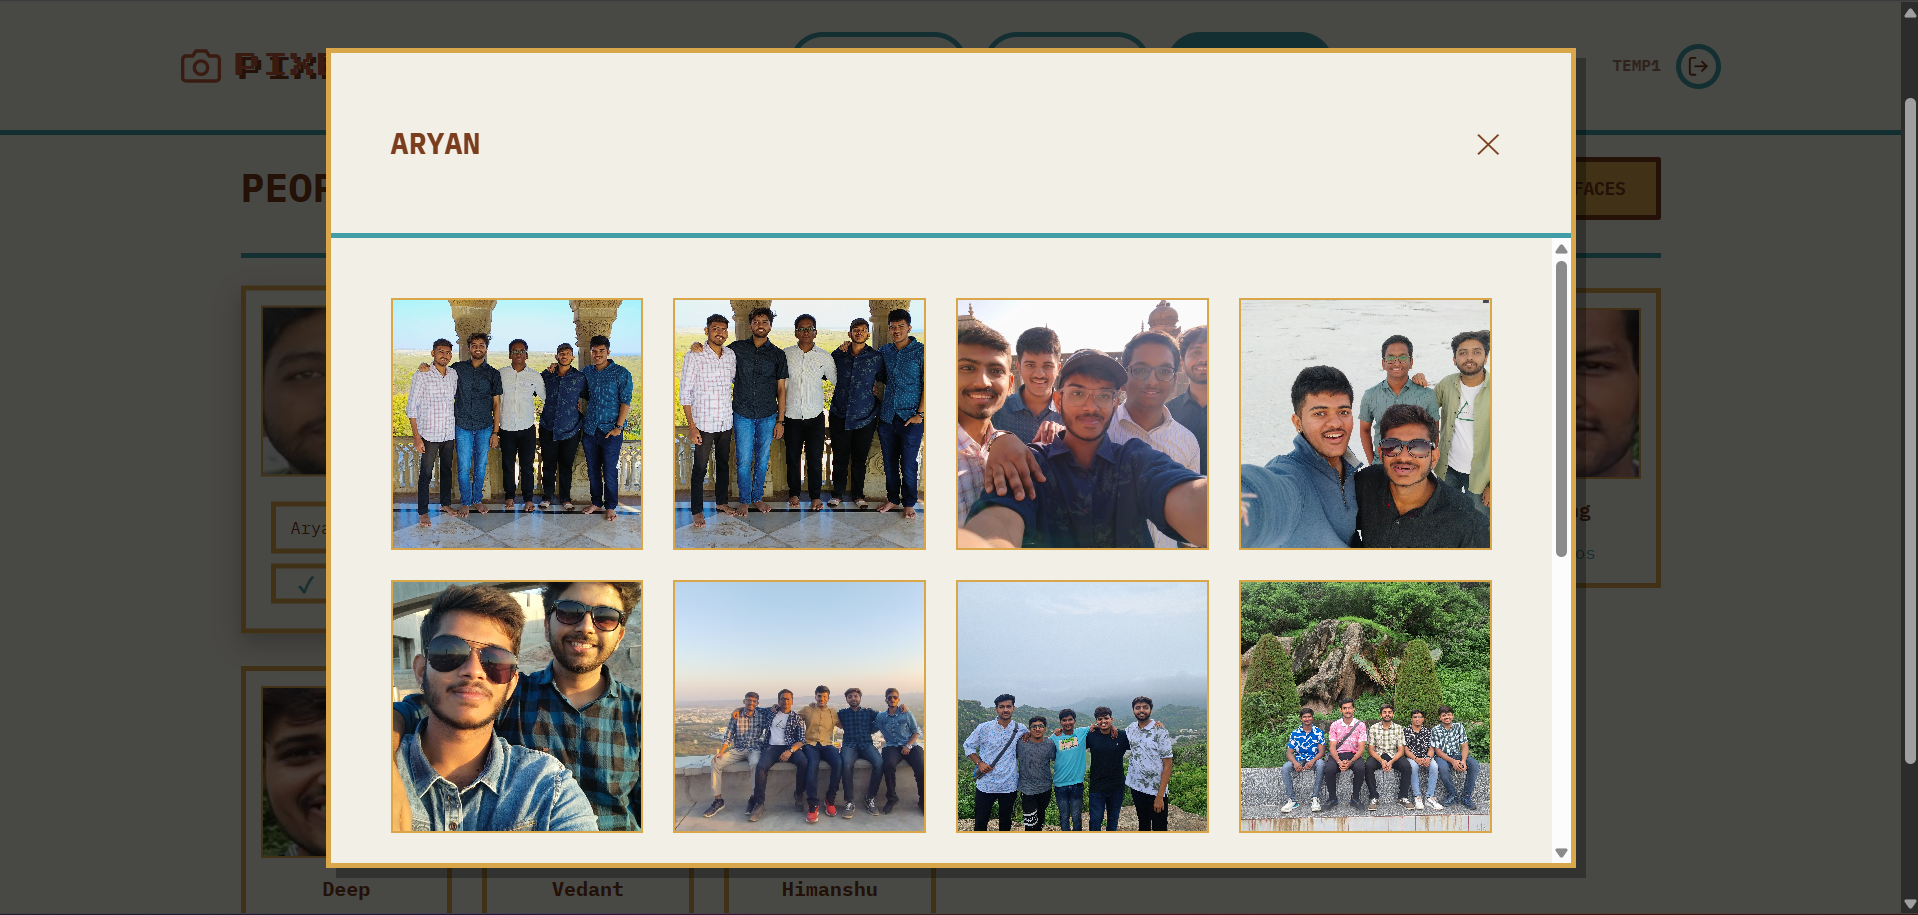
\includegraphics[width=\linewidth]{screenshots/FaceClustersImages.png}
\caption{Detailed view of all images associated with a specific person}
\label{fig:ss-faces-detail}
\end{figure}

\begin{figure}[H]
\centering
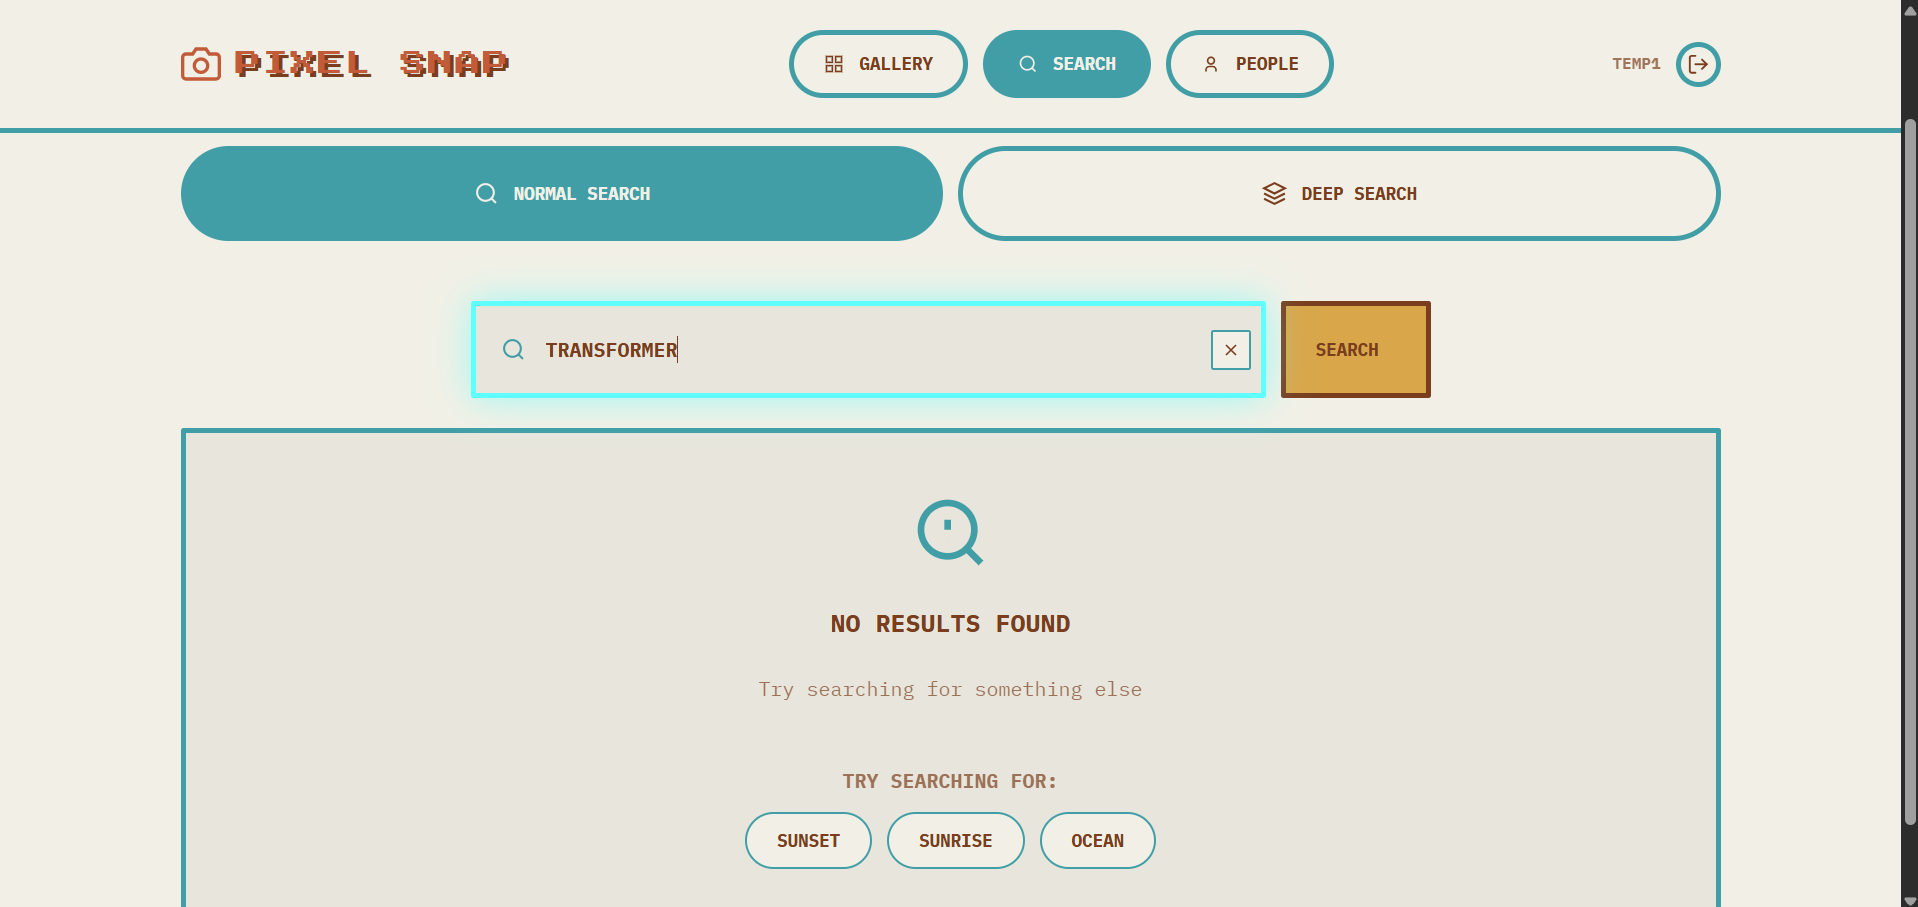
\includegraphics[width=\linewidth]{screenshots/NoResults.png}
\caption{Search interface displaying the fallback state when no
  matching results are found}
\label{fig:ss-no-results}
\end{figure}

\section{Failure Analysis}

While the system generally performs exceptionally well for consumer image
collections, detailed testing revealed several failure cases that highlight the
inherent limitations of the underlying AI models:

\begin{enumerate}[leftmargin=*]
  \item \textbf{CLIP Concept Confusion}: CLIP embeddings occasionally fail to safely
        distinguish between closely related semantic concepts with similar visual structures.
        For example, a query for ``fox in the snow'' erroneously returned high-ranking
        images of an orange domestic cat. CLIP focuses heavily on broad concept presence
        rather than fine-grained taxonomy.
  \item \textbf{Incorrect Face Clustering}: The unsupervised DBSCAN clustering
        algorithm misclassified distinct individuals as the same person (false positive
        merges) when lighting conditions or facial angles were severely distorted. It also fractured 
        images of the same individual into separate clusters (false negative splits) if the 
        person appeared across vastly different age ranges (e.g., childhood vs. adulthood).
  \item \textbf{VLM Hallucinated Descriptions}: The SmolVLM model occasionally fabricated details 
        that were logically plausible but factually absent from the image. For instance, 
        upon analyzing a photograph of a cup of coffee on a wooden desk next to a blank notebook,
        SmolVLM generated a description stating: ``...a cup of coffee next to a notebook with 
        writing on it.'' These text hallucinations directly degrade the precision of the BM25 Deep Search mode.
\end{enumerate}

% ======================================================================
%  CHAPTER 7 — CONCLUSION
% ======================================================================
\chapter{Conclusion}

\section{Summary of Contributions}
This project designed, implemented, and deployed a full-stack AI-powered
image search platform, \textbf{Media-Search}, with the following
contributions:

\begin{enumerate}[leftmargin=*]
  \item \textbf{Multi-Modal Semantic Search:} A two-stage CLIP retrieval
        pipeline (ViT-L/14 global recall + local crop re-ranking) enabling
        accurate natural language image search without manual labelling.
  \item \textbf{Hybrid Search:} BM25 over SmolVLM-generated descriptions
        combined with CLIP semantic scoring, outperforming either signal
        alone for attribute-specific queries.
  \item \textbf{Automated Face Organisation:} End-to-end face detection and
        clustering (DeepFace + DBSCAN) allowing search by person name.
  \item \textbf{Secure Multi-User Architecture:} JWT authentication,
        bcrypt hashing, and per-user data isolation (filesystem + Qdrant
        payload filtering) supporting multiple concurrent users.
  \item \textbf{Real-Time Feedback:} Server-Sent Events infrastructure
        streaming live AI processing status to the React frontend.
  \item \textbf{Open, Self-Hosted Deployment:} A completely open-source
        system running on commodity hardware with Docker Compose.
\end{enumerate}

\section{Limitations}
\begin{itemize}[leftmargin=*]
  \item \textbf{High VRAM Requirement}: VLM description generation and face detection
        can be VRAM-intensive. Using CUDA acceleration on an entry-level GPU like the
        RTX 3050 drastically reduces times, but simultaneous large library uploads
        must be queued carefully to avoid out-of-memory (OOM) errors.
  \item \textbf{DBSCAN Clustering Errors}: The parameter-free nature of DBSCAN
        is advantageous, but fixing the hyperparameters ($\varepsilon$, \texttt{min\_samples})
        leads to unavoidable clustering errors (splitting or merging identities) when processing
        large, demographically diverse collections with overlapping facial embeddings.
  \item \textbf{Dependence on Pretrained Models}: The system's intelligence relies
        strictly on the pre-existing biases and capabilities of OpenAI's CLIP and
        HuggingFace's SmolVLM. It cannot dynamically "learn" new concepts that the 
        models did not encounter during their original web-scale training phase.
  \item Video content is not supported; only static images are indexed.
\end{itemize}

\section{Future Work}
\begin{itemize}[leftmargin=*]
  \item \textbf{Multi-GPU Scaling:} Distributing inference tasks across multiple
        GPUs to handle extremely large simultaneous upload streams in a multi-user environment.
  \item \textbf{Video Frame Search:} Keyframe extraction from video files
        and indexing in Qdrant would enable video content search.
  \item \textbf{Fine-Tuned CLIP:} Domain-specific fine-tuning on
        medical, satellite, or professional imagery would improve
        retrieval performance for specialised libraries.
  \item \textbf{Microservices Architecture:} Separating CLIP, VLM, and
        face services into independent containers with a message queue
        would enable independent scaling and zero-downtime updates.
  \item \textbf{Active Learning for Clustering:} Incorporating user
        feedback (merge/split clusters) into periodic DBSCAN
        re-clustering would improve identity grouping over time.
  \item \textbf{Mobile Client:} A React Native mobile app would allow
        on-device capture and direct upload from smartphones.
\end{itemize}

\section{Concluding Remarks}
Media-Search demonstrates that state-of-the-art AI image retrieval,
previously confined to resource-rich cloud providers, can be
delivered as a self-hosted, privacy-preserving application on a single
commodity server.  The integration of CLIP, SmolVLM, DeepFace, DBSCAN,
and Qdrant within a modular FastAPI backend produces a system that is
both technically sophisticated and practically useful.  The project
provides valuable hands-on experience in vector database technology,
asynchronous Python web development, multi-modal AI integration, and
modern React frontend engineering, and lays a solid foundation for
the future extensions described above.

% ======================================================================
%  REFERENCES
% ======================================================================
\chapter*{References}
\addcontentsline{toc}{chapter}{References}

\begin{enumerate}[label={[\arabic*]}, leftmargin=2.2em]

\item A.~Radford, J.~W.~Kim, C.~Hallacy et~al.,
  ``Learning Transferable Visual Models From Natural Language
  Supervision,''
  in \textit{Proc.\ ICML}, pp.~8748--8763, 2021.

\item A.~Dosovitskiy, L.~Beyer, A.~Kolesnikov et~al.,
  ``An Image is Worth 16$\times$16 Words: Transformers for Image
  Recognition at Scale,''
  in \textit{Proc.\ ICLR}, 2021.

\item G.~Ilharco, M.~Wortsman, R.~Wightman et~al.,
  ``OpenCLIP,''
  \textit{Zenodo}, 2021.
  [Online]. Available: \url{https://doi.org/10.5281/zenodo.5143773}

\item X.~Zhai, B.~Mustafa, A.~Kolesnikov, and L.~Beyer,
  ``Sigmoid Loss for Language Image Pre-Training,''
  in \textit{Proc.\ ICCV}, pp.~11975--11986, 2023.

\item HuggingFace,
  ``SmolVLM: Small Vision Language Model,''
  \textit{HuggingFace Hub}, 2024.
  [Online]. Available: \url{https://huggingface.co/HuggingFaceTB/SmolVLM-Instruct}

\item P.~Viola and M.~Jones,
  ``Rapid object detection using a boosted cascade of simple features,''
  in \textit{Proc.\ IEEE CVPR}, vol.~1, pp.~511--518, 2001.

\item S.~Serengil and A.~Ozpinar,
  ``DeepFace: A Lightweight Face Recognition and Facial Attribute
  Analysis Framework for Python,''
  in \textit{Proc.\ IEEE INNS EANN}, 2021.

\item M.~Ester, H.-P.~Kriegel, J.~Sander, and X.~Xu,
  ``A Density-Based Algorithm for Discovering Clusters in Large Spatial
  Databases with Noise,''
  in \textit{Proc.\ KDD}, pp.~226--231, 1996.

\item Y.~A.~Malkov and D.~A.~Yashunin,
  ``Efficient and Robust Approximate Nearest Neighbor Search Using
  Hierarchical Navigable Small World Graphs,''
  \textit{IEEE Trans.\ PAMI}, vol.~42, no.~4, pp.~824--836, 2020.

\item Qdrant Team,
  ``Qdrant: High-Performance Vector Search Engine,''
  \textit{GitHub}, 2023.
  [Online]. Available: \url{https://github.com/qdrant/qdrant}

\item S.~E.~Robertson and S.~Walker,
  ``Some Simple Effective Approximations to the 2-Poisson Model for
  Probabilistic Weighted Retrieval,''
  in \textit{Proc.\ ACM SIGIR}, pp.~232--241, 1994.

\item V.~Karpukhin, B.~Oguz, S.~Min et~al.,
  ``Dense Passage Retrieval for Open-Domain Question Answering,''
  in \textit{Proc.\ EMNLP}, pp.~6769--6781, 2020.

\end{enumerate}

% ======================================================================
%  ABBREVIATIONS
% ======================================================================
\chapter*{List of Abbreviations}
\addcontentsline{toc}{chapter}{List of Abbreviations}

\begin{longtable}{p{3.2cm} p{10.5cm}}
\textbf{AI}     & Artificial Intelligence \\
\textbf{ANN}    & Approximate Nearest Neighbour \\
\textbf{API}    & Application Programming Interface \\
\textbf{BM25}   & Best Match 25 \\
\textbf{CBIR}   & Content-Based Image Retrieval \\
\textbf{CLIP}   & Contrastive Language-Image Pre-training \\
\textbf{CNN}    & Convolutional Neural Network \\
\textbf{CORS}   & Cross-Origin Resource Sharing \\
\textbf{CUDA}   & Compute Unified Device Architecture \\
\textbf{DBSCAN} & Density-Based Spatial Clustering of Applications with Noise \\
\textbf{DFD}    & Data Flow Diagram \\
\textbf{ER}     & Entity-Relationship \\
\textbf{FR}     & Functional Requirement \\
\textbf{GPU}    & Graphics Processing Unit \\
\textbf{GTU}    & Gujarat Technological University \\
\textbf{HNSW}   & Hierarchical Navigable Small World \\
\textbf{HTML}   & HyperText Markup Language \\
\textbf{HTTP}   & HyperText Transfer Protocol \\
\textbf{HTTPS}  & HyperText Transfer Protocol Secure \\
\textbf{JWT}    & JSON Web Token \\
\textbf{ML}     & Machine Learning \\
\textbf{NFR}    & Non-Functional Requirement \\
\textbf{ORM}    & Object-Relational Mapper \\
\textbf{REST}   & Representational State Transfer \\
\textbf{SPA}    & Single Page Application \\
\textbf{SQL}    & Structured Query Language \\
\textbf{SSE}    & Server-Sent Events \\
\textbf{TF-IDF} & Term Frequency -- Inverse Document Frequency \\
\textbf{UUID}   & Universally Unique Identifier \\
\textbf{VGEC}   & Vishwakarma Government Engineering College \\
\textbf{ViT}    & Vision Transformer \\
\textbf{VLM}    & Vision-Language Model \\
\end{longtable}

\end{document}


